\documentclass{article}
\usepackage[utf8]{inputenc} %кодировка
\usepackage[T2A]{fontenc}
\usepackage[english,russian]{babel} %русификатор 
\usepackage{mathtools} %библиотека матеши
\usepackage[left=1cm,right=1cm,top=2cm,bottom=2cm,bindingoffset=0cm]{geometry} %изменение отступов на листе
\usepackage{amsmath}
\usepackage{graphicx} %библиотека для графики и картинок
\graphicspath{}
\DeclareGraphicsExtensions{.pdf,.png,.jpg}
\usepackage{subcaption}
\usepackage{pgfplots}
\usepackage{float}
\usepackage{listings}
\usepackage{hyperref}
\usepackage{physics}
\usepackage{xcolor}

% Настройки отображения кода
\lstset{
    basicstyle=\ttfamily\small,
    breaklines=true, % Включить перенос строк
    postbreak=\mbox{\textcolor{red}{$\hookrightarrow$}\space}, % Маркер переноса строки
    frame=single, % Рамка вокруг кода
    numbers=left, % Номера строк слева
    numberstyle=\tiny\color{gray}, % Стиль номеров строк
    keywordstyle=\color{blue}, % Стиль ключевых слов
    commentstyle=\color{gray}, % Стиль комментариев
    stringstyle=\color{purple} % Стиль строк
}

\begin{document}
% НАЧАЛО ТИТУЛЬНОГО ЛИСТА
\begin{center}
    \Large
    Федеральное государственное автономное \\
    образовательное учреждение высшего образования \\ 
    «Научно-образовательная корпорация ИТМО»\\
    \vspace{0.5cm}
    \large
    Факультет программной инженерии и компьютерной техники \\
    Направление подготовки 09.03.04 Программная инженерия \\
    \vspace{1cm}
    \Large
    \textbf{Отчёт по лабораторной работе №4} \\
    По дисциплине «Основы Программной Инженерии» (4 семестр)\\
    \large
    \vspace{8cm}

    \begin{minipage}{.33\textwidth}
    \end{minipage}
    \hfill
    \begin{minipage}{.4\textwidth}
    
        \textbf{Студенты}: \vspace{.1cm} \\
        \ Дениченко Александр P3212\\
        \ Беляев Михаил P3212\\
        \textbf{Практик}:  \\
        \ Осипов Святослав Владимирович
    \end{minipage}
    \vfill
Санкт-Петербург\\ 2024 г.
\end{center}
\pagestyle{empty}
% КОНЕЦ ТИТУЛЬНОГО ЛИСТА 
\newpage
\pagestyle{plain}
\section{Задание}
1. Для своей программы из лабораторной работы 3 по дисциплине "Веб-программирование" реализовать:

MBean, считающий общее число установленных пользователем точек, а также число точек, не попадающих в область. В случае, если пользователь совершил 2 "промаха" подряд, разработанный MBean должен отправлять оповещение об этом событии.

MBean, определяющий средний интервал между кликами пользователя по координатной плоскости.
\\ \\
2. С помощью утилиты JConsole провести мониторинг программы:

Снять показания MBean-классов, разработанных в ходе выполнения задания 1.
Определить версию Java Language Specification, реализуемую данной средой исполнения.
\\ \\
3. С помощью утилиты VisualVM провести мониторинг и профилирование программы:

Снять график изменения показаний MBean-классов, разработанных в ходе выполнения задания 1, с течением времени.
Определить имя класса, объекты которого занимают наибольший объём памяти JVM; определить пользовательский класс, в экземплярах которого находятся эти объекты.
\\ \\
4. С помощью утилиты VisualVM и профилировщика IDE NetBeans, Eclipse или Idea локализовать и устранить проблемы с производительностью в программе. По результатам локализации и устранения проблемы необходимо составить отчёт, в котором должна содержаться следующая информация:

Описание выявленной проблемы.

Описание путей устранения выявленной проблемы.

Подробное (со скриншотами) описание алгоритма действий, который позволил выявить и локализовать проблему.
\section{Исходный код разработанных MBean-классов}

\begin{lstlisting}[caption={Класс для подсчёта интервалов}]
@Getter
@Setter
@ManagedBean(name = "interval", eager = true)
@SessionScoped
public class ClickIntervalBean implements ClickIntervalBeanMBean, MBeanRegistration {
    private static final Logger logger = Logger.getLogger(ClickIntervalBean.class.getName());

    private List<Long> clickTimestamps = new LinkedList<>();
    private double averageInterval = 0;

    @Override
    public void addClickTimestamp() {
        long currentTime = System.currentTimeMillis();
        if (!clickTimestamps.isEmpty()) {
            long lastTime = clickTimestamps.get(clickTimestamps.size() - 1);
            averageInterval = ((averageInterval * (clickTimestamps.size() - 1)) + (currentTime - lastTime)) / clickTimestamps.size();
        }
        clickTimestamps.add(currentTime);
        logger.info("New click timestamp added: " + currentTime + "; Updated average interval: " + averageInterval);
    }

    @Override
    public void postRegister(Boolean registrationDone) {
        logger.info("ClickIntervalBean registered to the MBean server: " + registrationDone);
    }

    @Override
    public void postDeregister() {
        logger.info("ClickIntervalBean deregistered from the MBean server");
    }

    @Override
    public void preDeregister() {
        logger.info("ClickIntervalBean is about to be deregistered from the MBean server");
    }

    @Override
    public ObjectName preRegister(MBeanServer server, ObjectName name) throws Exception {
        // Optionally modify the name
        return name;
    }
}
\end{lstlisting}

\begin{lstlisting}[caption={Класс для подсчёта количества кликов}]
@Getter
@Setter
@ManagedBean(name = "counter", eager = true)
public class CounterBean implements CounterBeanMBean {
    private static final Logger logger = Logger.getLogger(CounterBean.class.getName());

    private int countHits;
    private int loseHits;
    private boolean lastHit;

    public CounterBean() {
        countHits = 0;
        loseHits = 0;
        lastHit = true;
    }

    @Override
    public void addHit(boolean res) {
        countHits++;
        if (!res) {
            loseHits++;
            if (!lastHit) {
                logger.info("2");
            }
        }
        lastHit = res;
    }

    @Override
    public int getCountHits() {
        return countHits;
    }

    @Override
    public int getLoseHits() {
        return loseHits;
    }

    @Override
    public boolean isLastHit() {
        return lastHit;
    }
}
\end{lstlisting}


\begin{lstlisting}[caption={Класс выступающий главным бином}]
@Getter
@Setter
@Named(value = "user")
@ApplicationScoped
public class UserDataBean {
    private static final Logger logger = Logger.getLogger(UserDataBean.class.getName());

    @Inject
    private CounterBean counterBean;
    @Inject
    private ClickIntervalBean clickIntervalBean;
    private Double x = (double) 0;
    private Double y = (double) 0;
    private Double r = (double) 0;
    private Boolean hit;
    private List<UserData> resultList;

    @PostConstruct
    public void init() {
        MBeanServer mbs = ManagementFactory.getPlatformMBeanServer();

        try {
            ObjectName nameCounter = new ObjectName("UserDataBean:name=CounterBean");
            mbs.registerMBean(counterBean, nameCounter);

            ObjectName nameInterval = new ObjectName("UserDataBean:name=ClickIntervalBean");
            mbs.registerMBean(clickIntervalBean, nameInterval);
        } catch (Exception e) {
            e.printStackTrace();
        }
        logger.info("JConsole for manage");
    }


    private void updateLocal() {
        SessionFactory sessionFactory = HibernateUtil.getSessionFactory();
        UserDataDao userDataDao = new UserDataDao(sessionFactory);
        resultList = userDataDao.getUserData();
    }
    public void clearTable(){
        SessionFactory sessionFactory = HibernateUtil.getSessionFactory();
        UserDataDao userDataDao = new UserDataDao(sessionFactory);
        userDataDao.clearResultTable();
        updateLocal();
    }

    public void saveData() {
        if ((x >= 0 && x <= r / 2) && (y >= 0 && y <= r)){
            hit = true;}
        else if ((x <= 0 && x >= -r) && (y <= 0 && y >=  -r/2)){
            hit = (x>=-r-2*y);}
        else if ((x >= 0 && x <= r) && (y <= 0 && y >= -r)){
            hit = (Math.pow(x, 2) + Math.pow(y, 2) <= Math.pow(r, 2));}
        else{
            hit = false;}
        if(r==0){
            hit = false;
        }

        if (x == null) {
            x = (double) 0;
        } else if (!(x instanceof Number)) {
            x = (double) 0;
        }
        if (y == null) {
            y = (double) 0;
        } else if (!(y instanceof Number)) {
            y = (double) 0;
        }
        if (r == null) {
            r = (double) 0;
        } else if (!(r instanceof Number)) {
            r = (double) 0;
        }

        counterBean.addHit(hit);
        clickIntervalBean.addClickTimestamp();
        logger.info(String.valueOf(clickIntervalBean.getAverageInterval()));

        SessionFactory sessionFactory = HibernateUtil.getSessionFactory();
        UserDataDao userDataDao = new UserDataDao(sessionFactory);
        userDataDao.saveUserData(x, y, r, hit);
        updateLocal();
    }
}
\end{lstlisting}

\section{Снятые показания в ходе мониторинга}
\begin{center}
    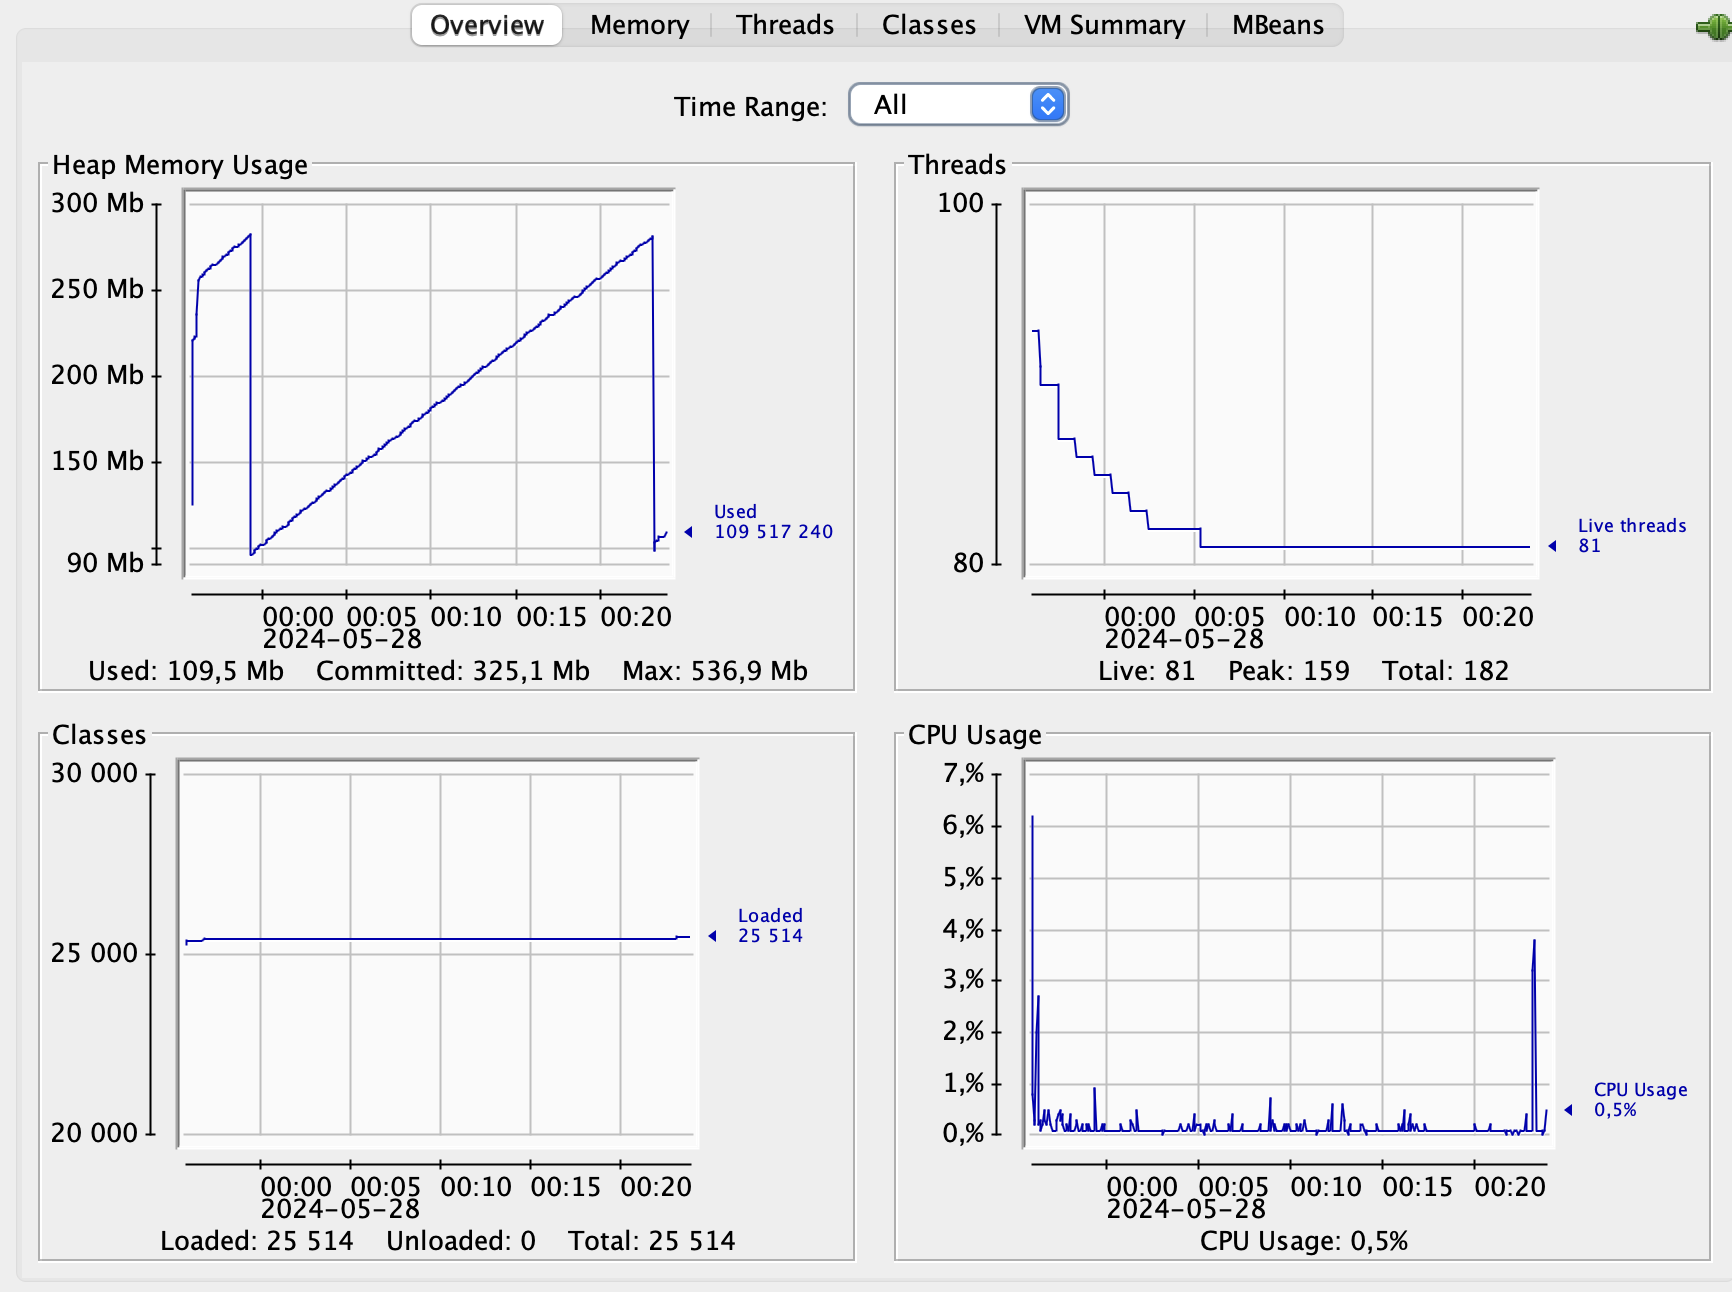
\includegraphics[width=.8\textwidth]{overview.png}\\
    \textbf{Скриншот 1. Общий вид}
\end{center}

\begin{center}
    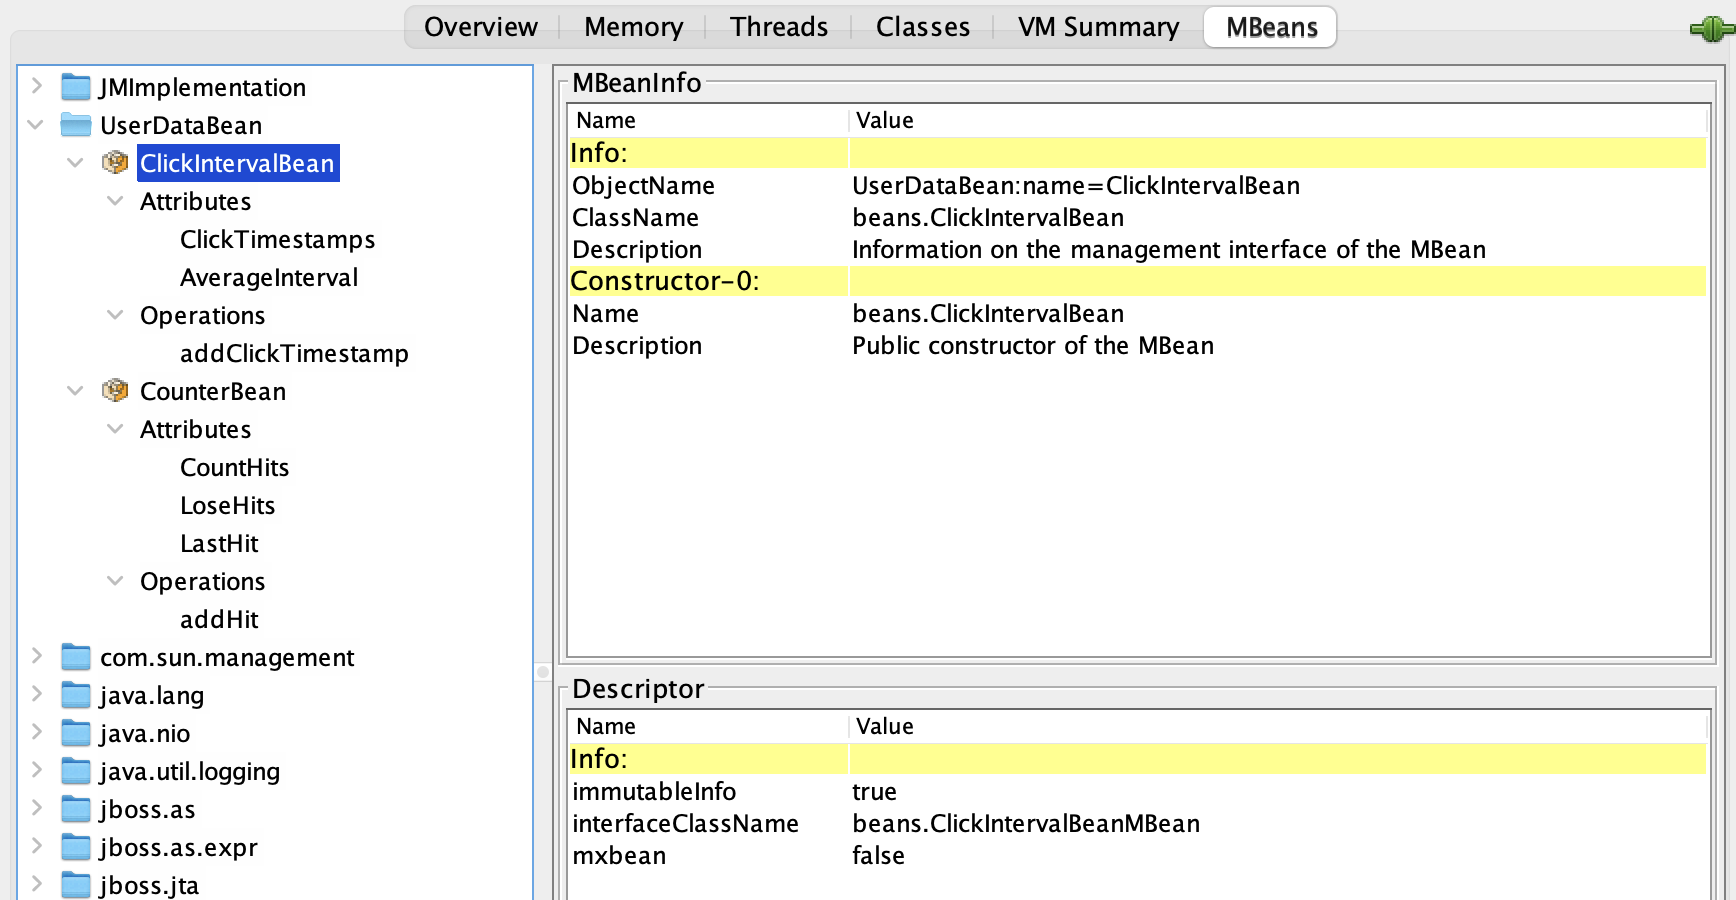
\includegraphics[width=.8\textwidth]{interval.png}\\
    \textbf{Скриншот 2. Бин интервал}
\end{center}

\begin{center}
    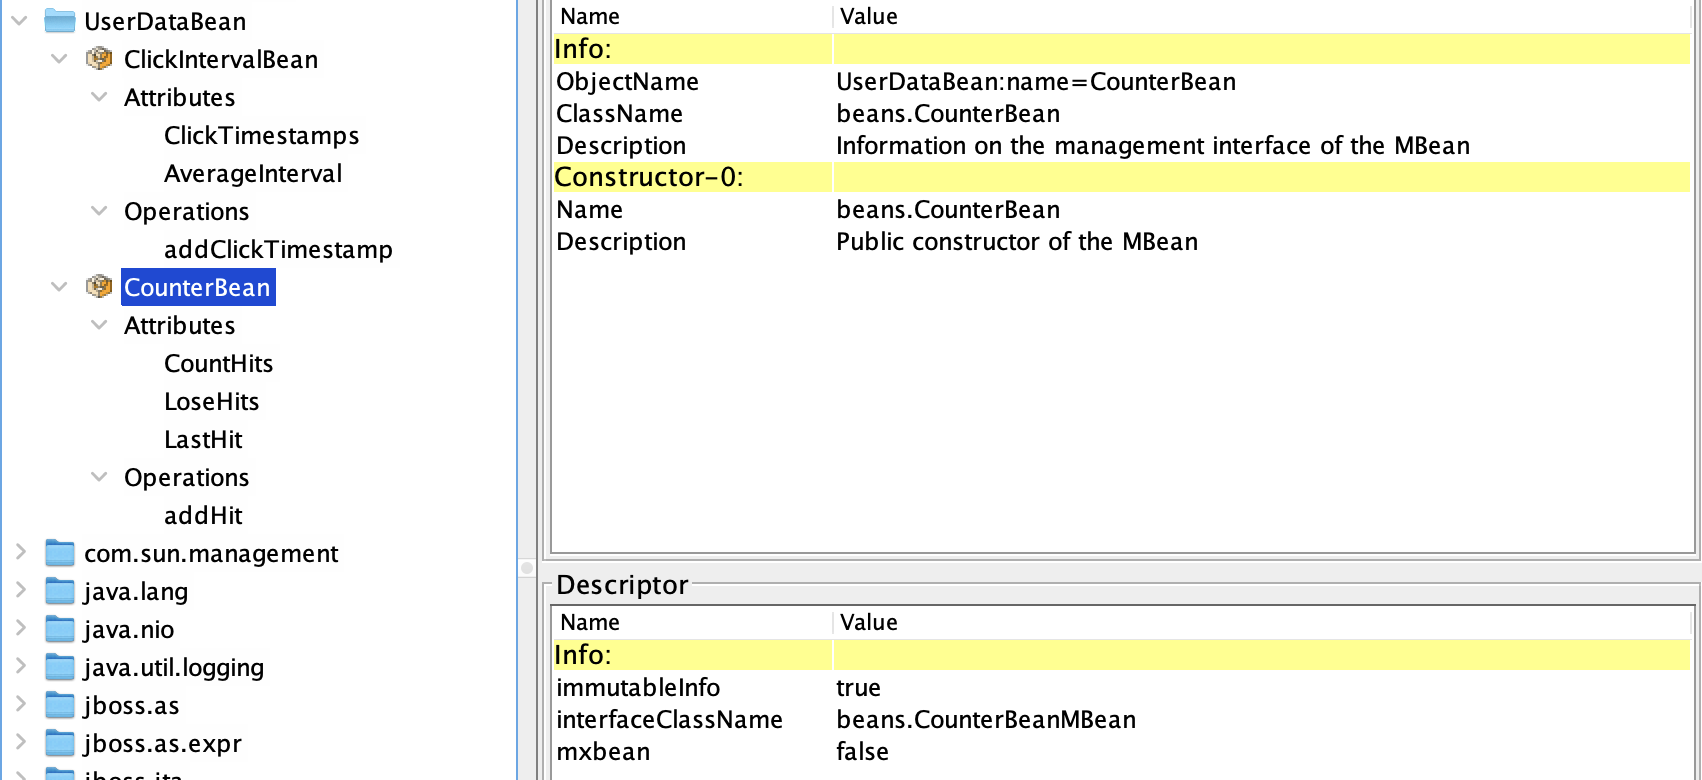
\includegraphics[width=.8\textwidth]{click.png}\\
    \textbf{Скриншот 3. Клик бин}
\end{center}

\begin{center}
    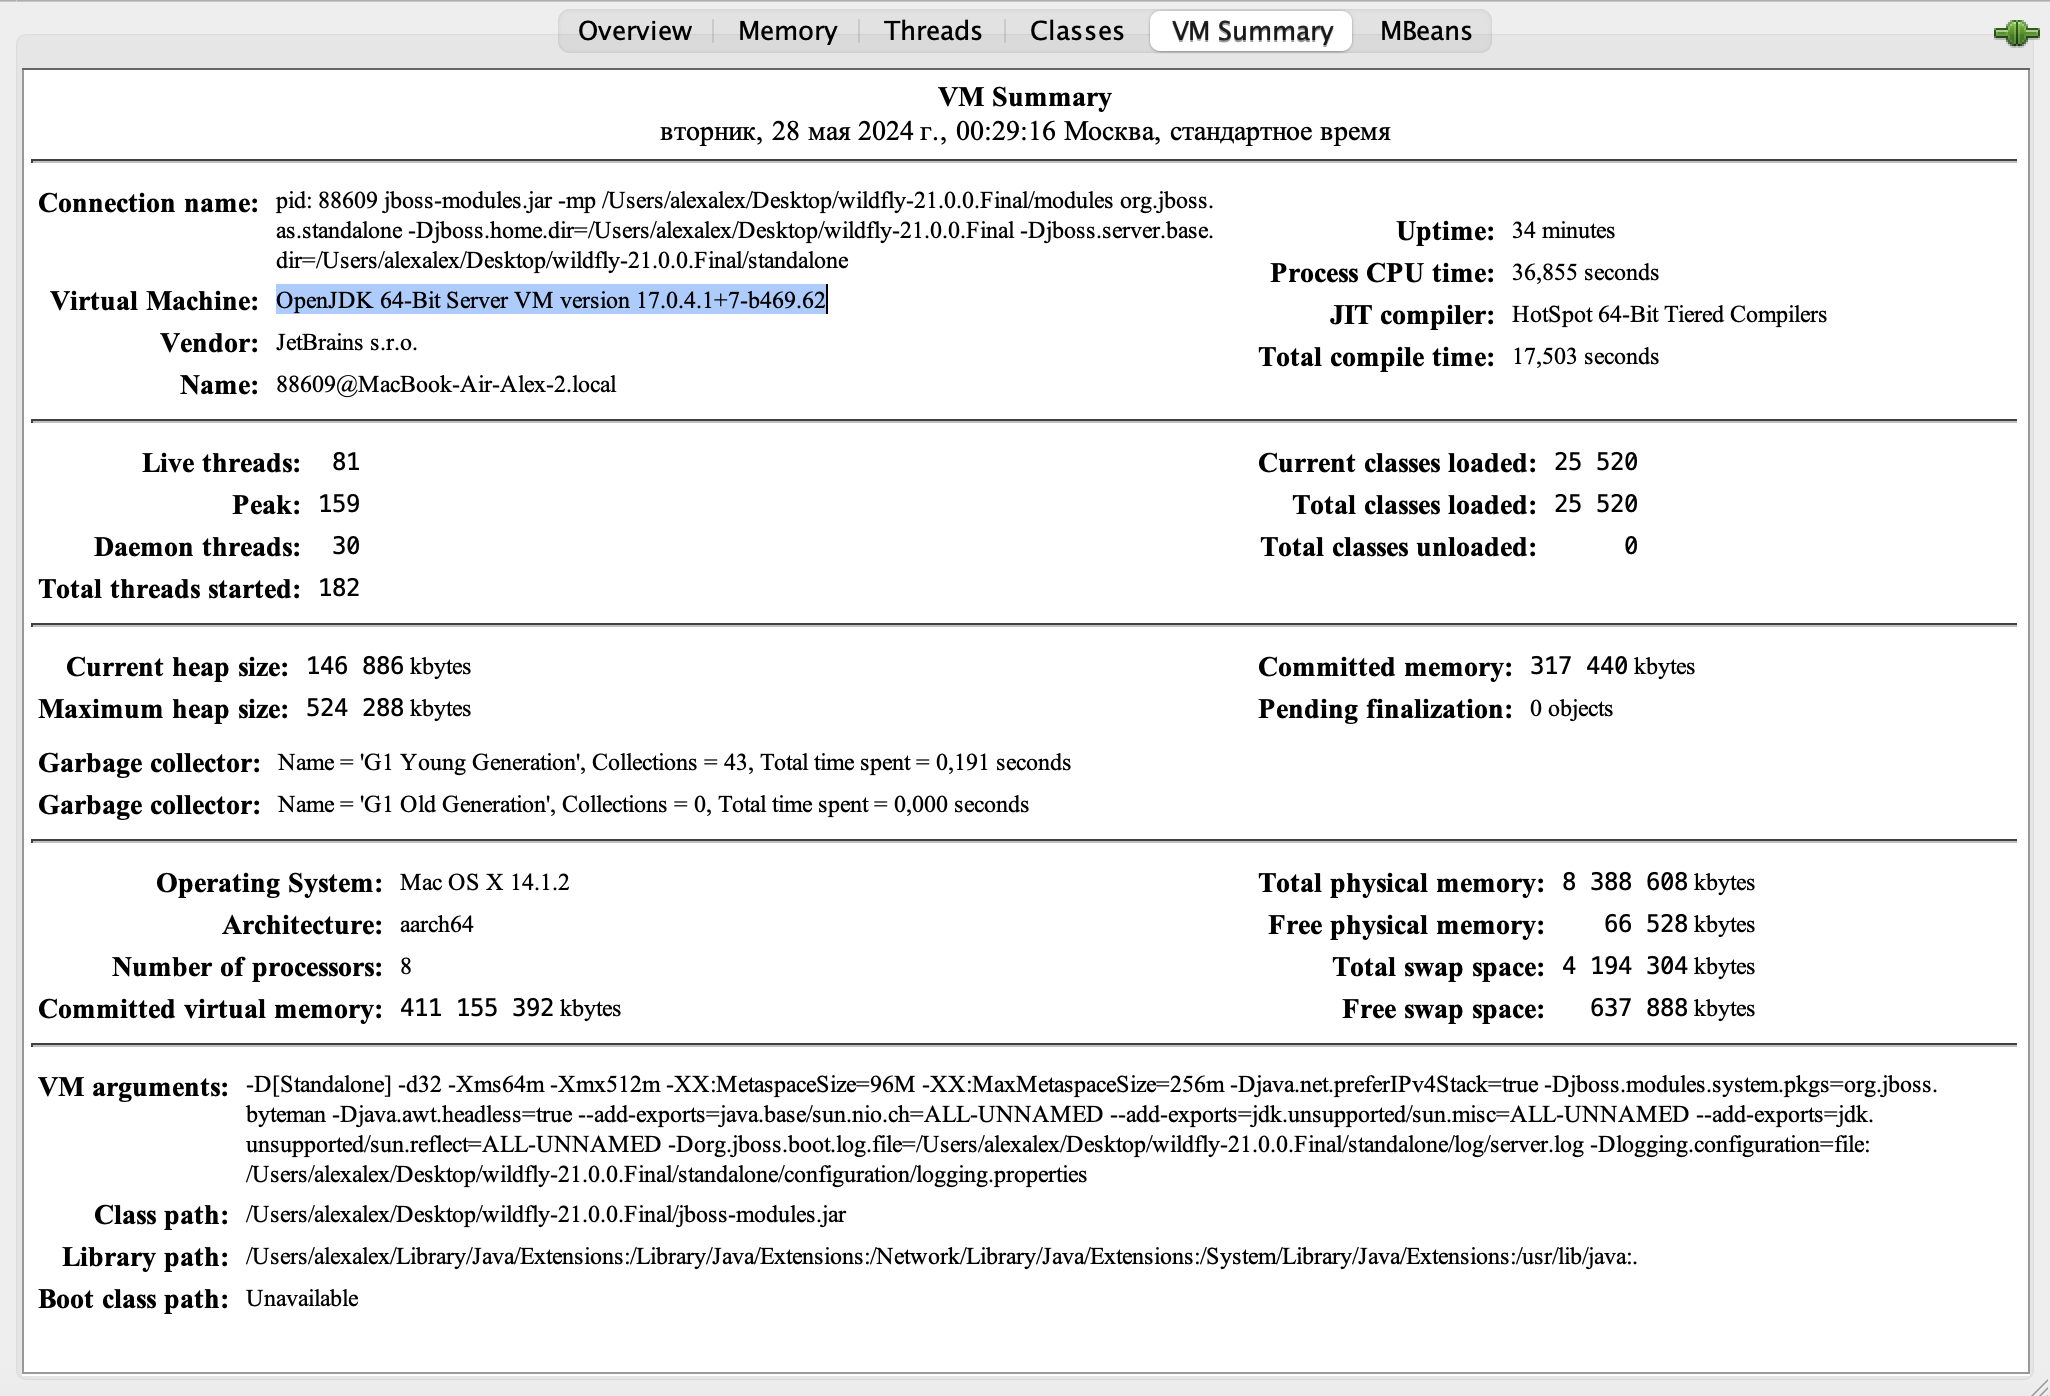
\includegraphics[width=.8\textwidth]{version.png}\\
    \textbf{Скриншот 4. Версия}
\end{center}

\begin{center}
    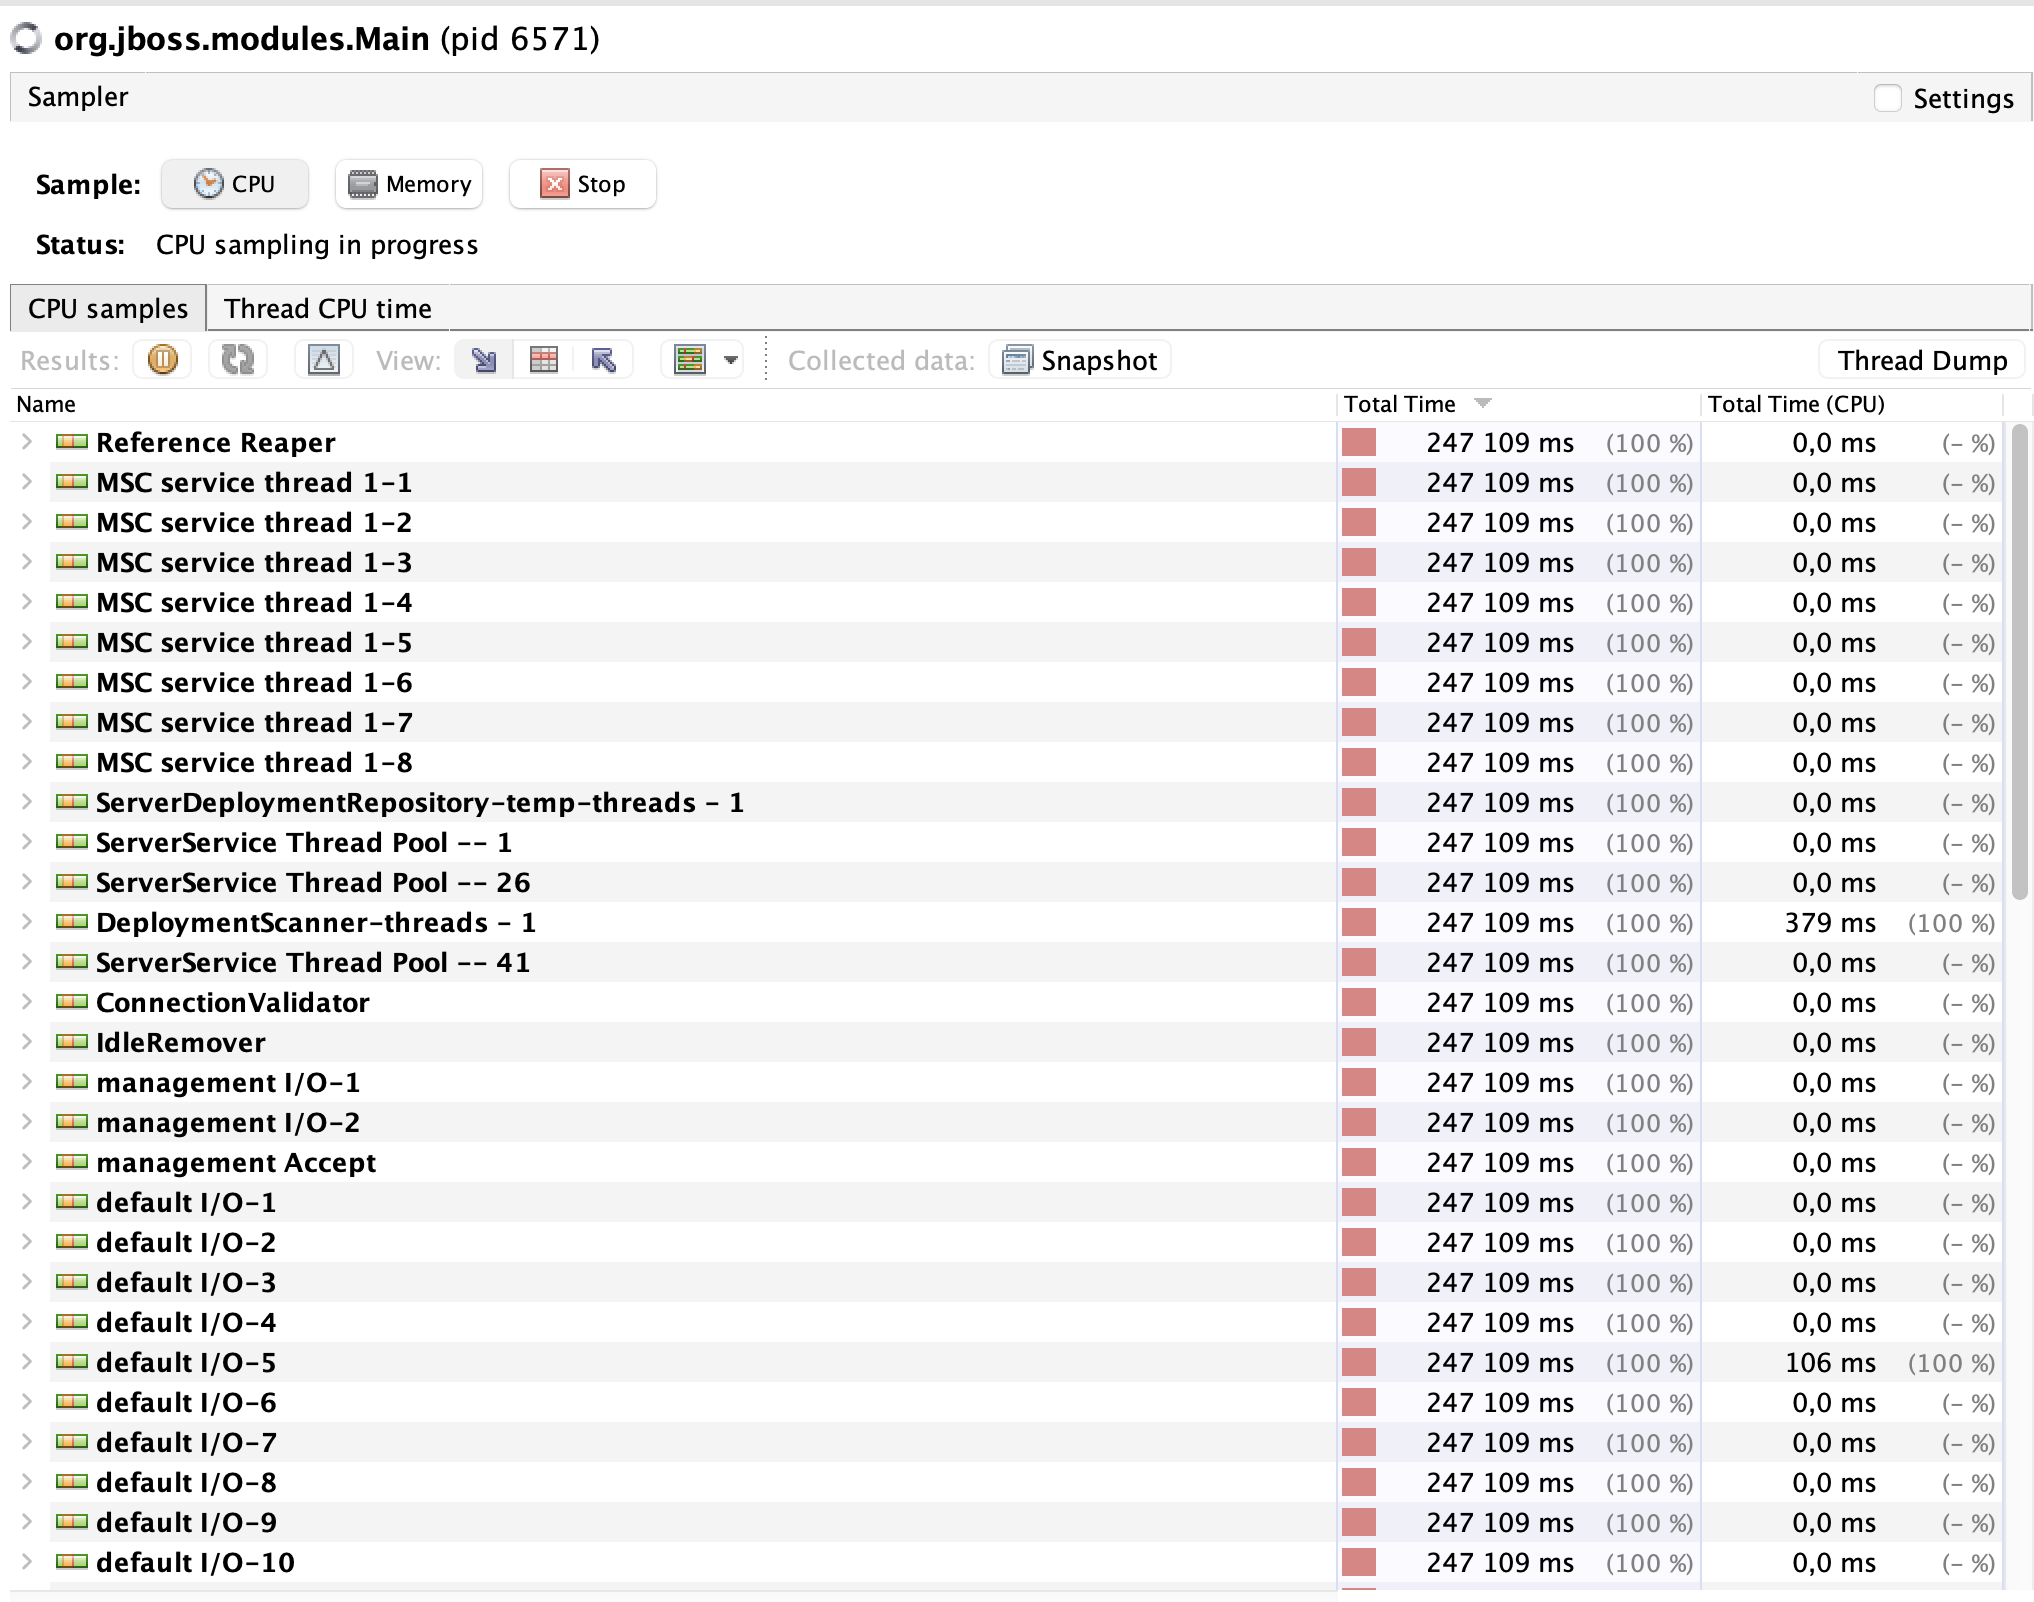
\includegraphics[width=.9\textwidth]{visualVM.png}\\
    \textbf{Скриншот 5. Показания VisualVM}
\end{center}

\begin{center}
    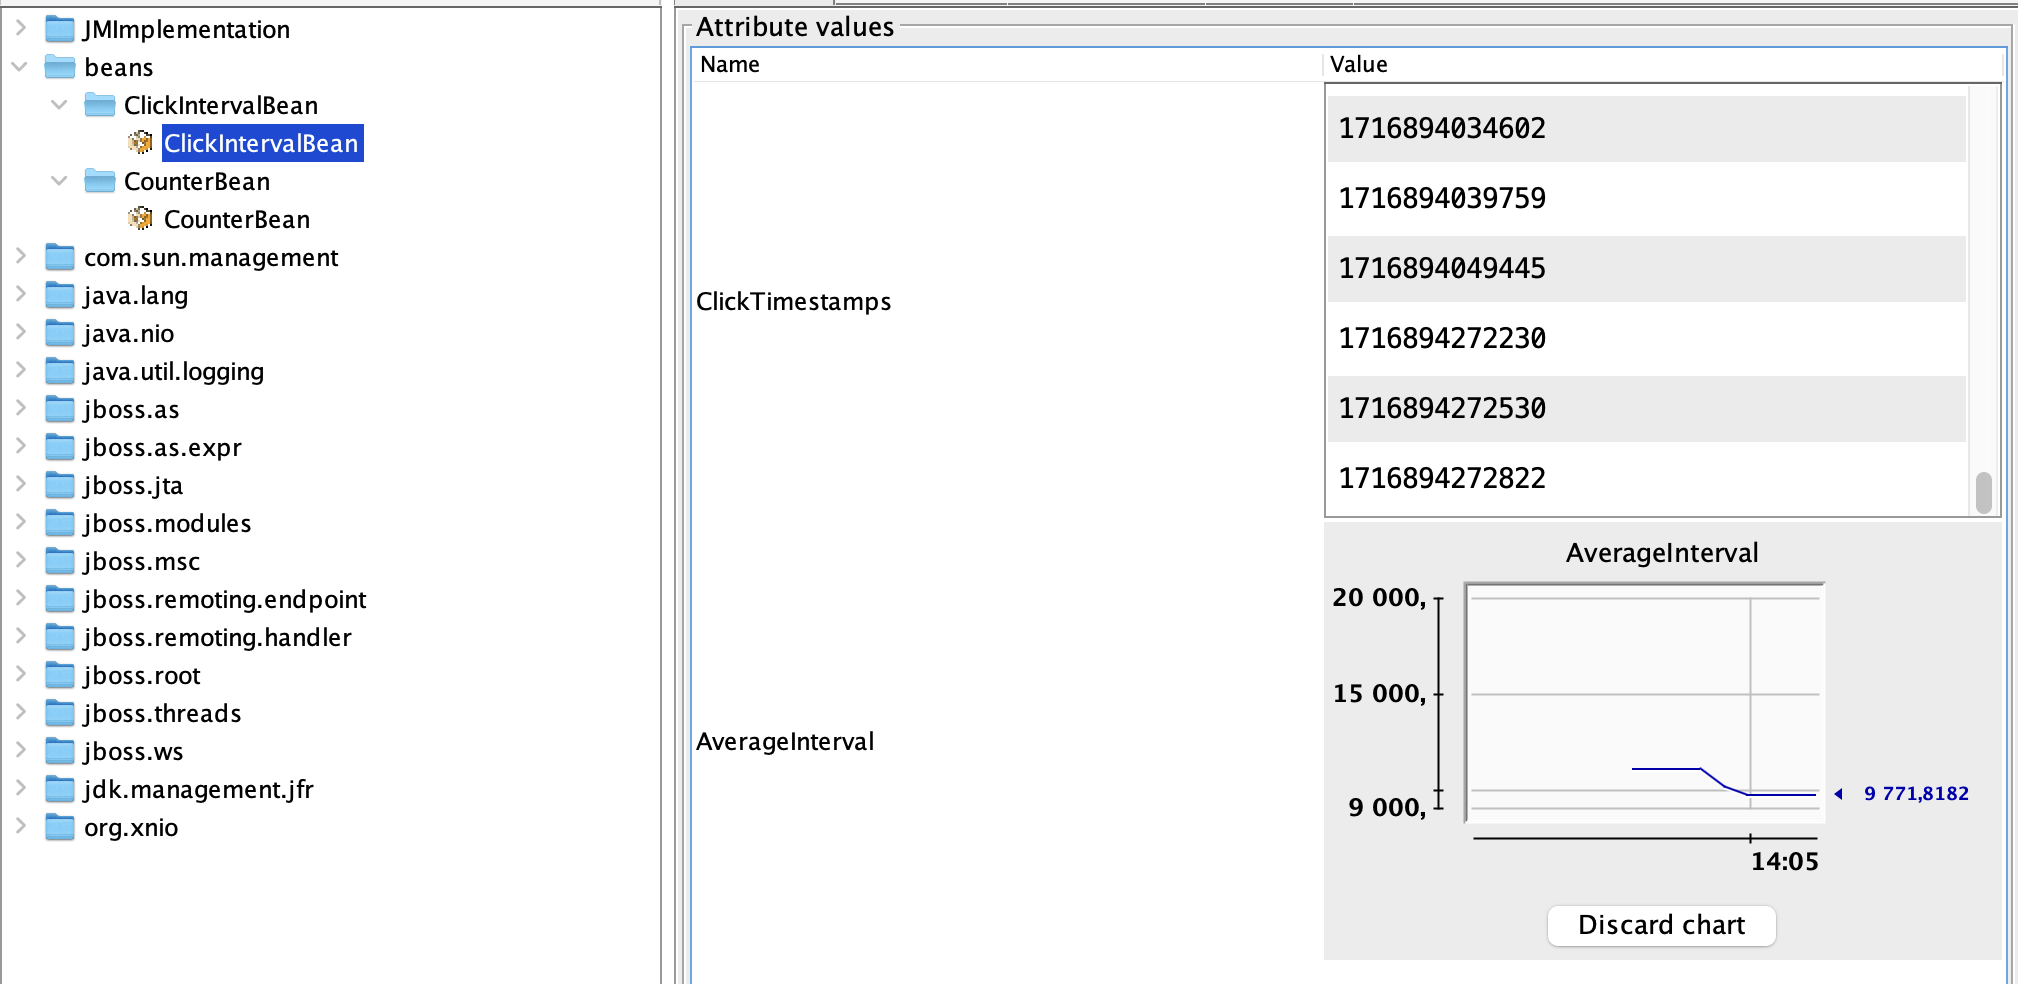
\includegraphics[width=.9\textwidth]{interChart.png}\\
    \textbf{Скриншот 6. Показания VisualVM для интервального бина}
\end{center}

\begin{center}
    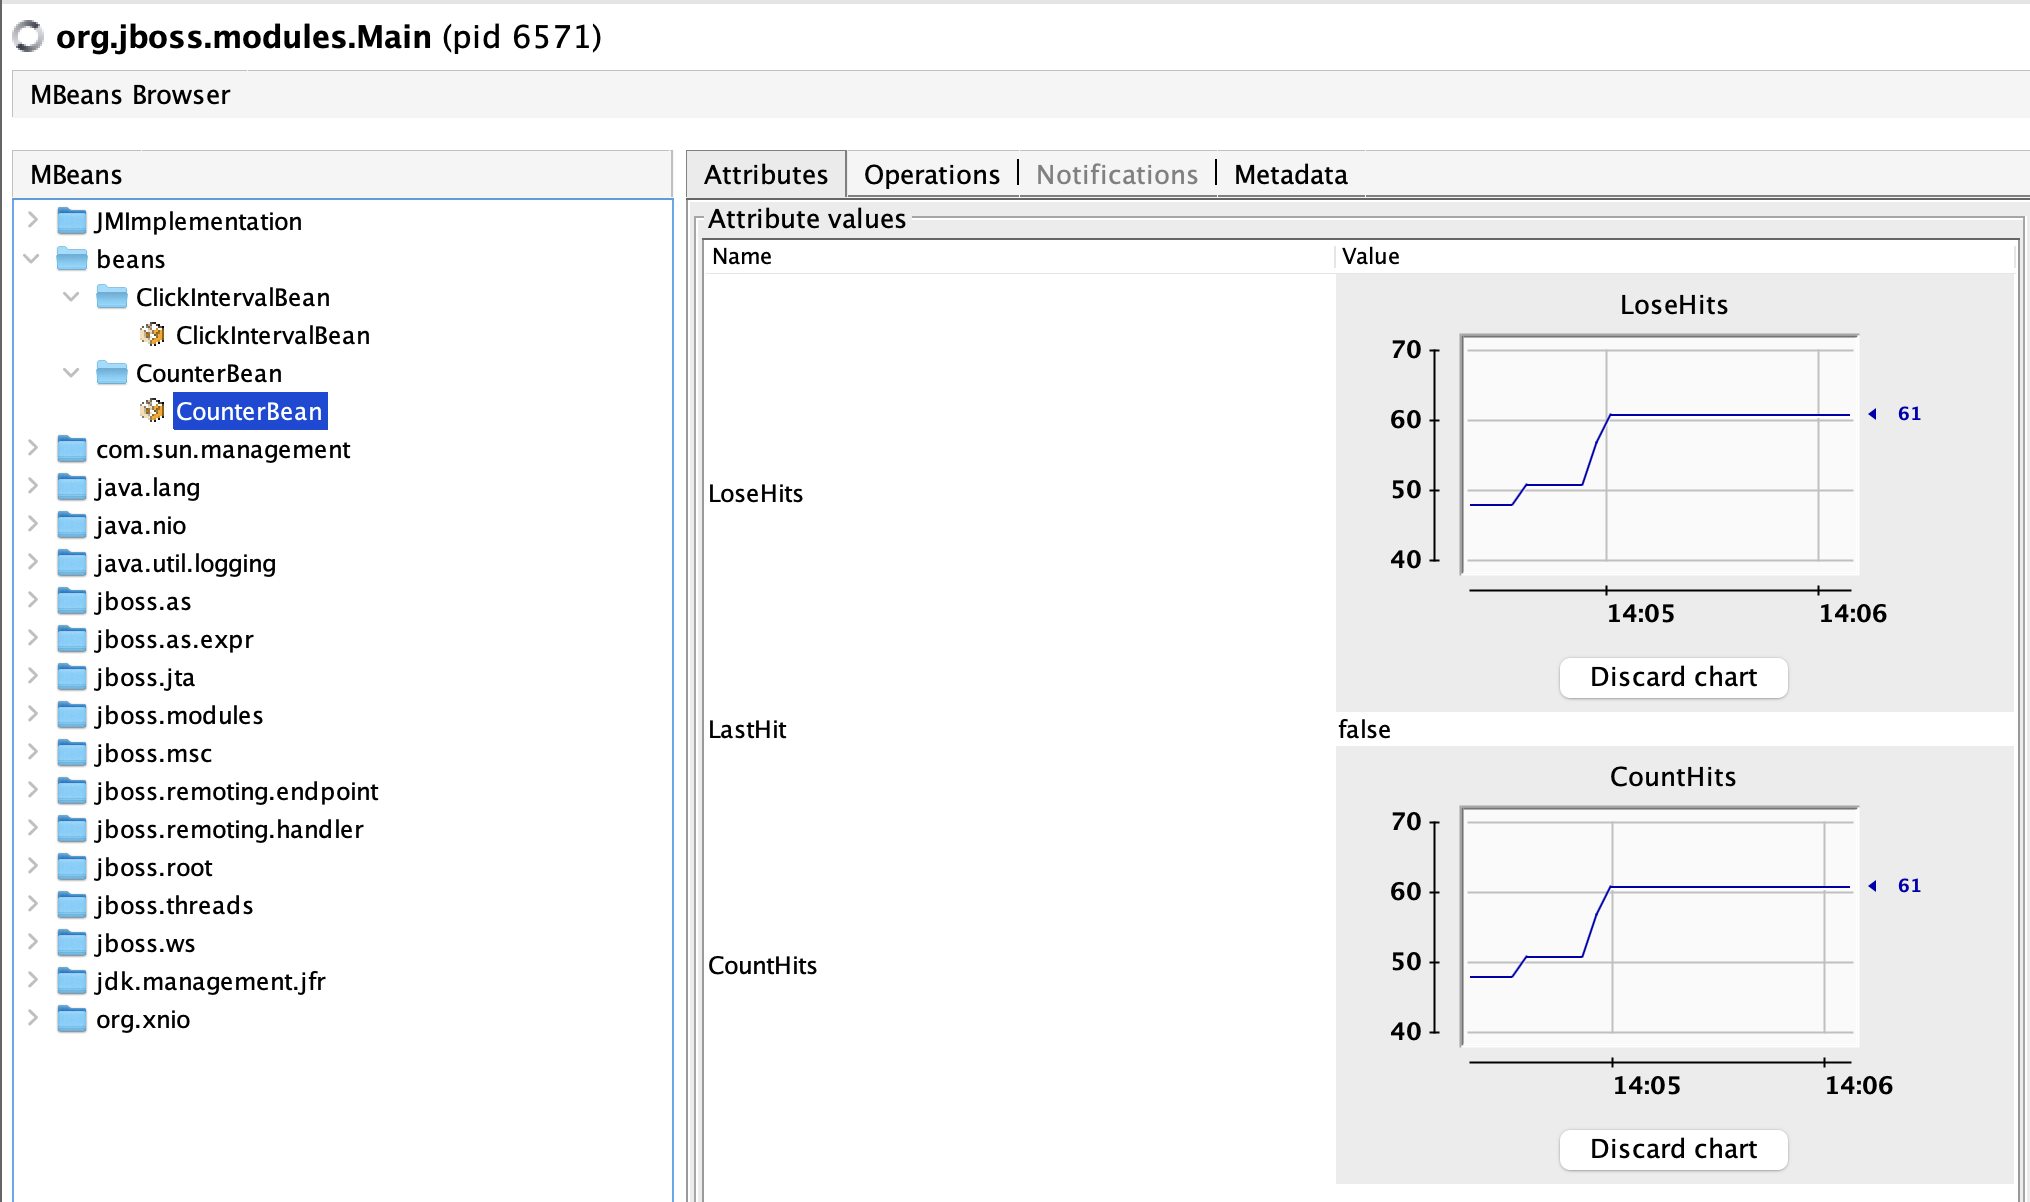
\includegraphics[width=.9\textwidth]{countBB.png}\\
    \textbf{Скриншот 7. Показания VisualVM для количественного бина}
\end{center}

\section{Проверка кода на утечки памяти}
Нашли цикл, где поменяли время сна на 0, а так же выставили максмаильный размер кучи 50МВ.
\begin{center}
    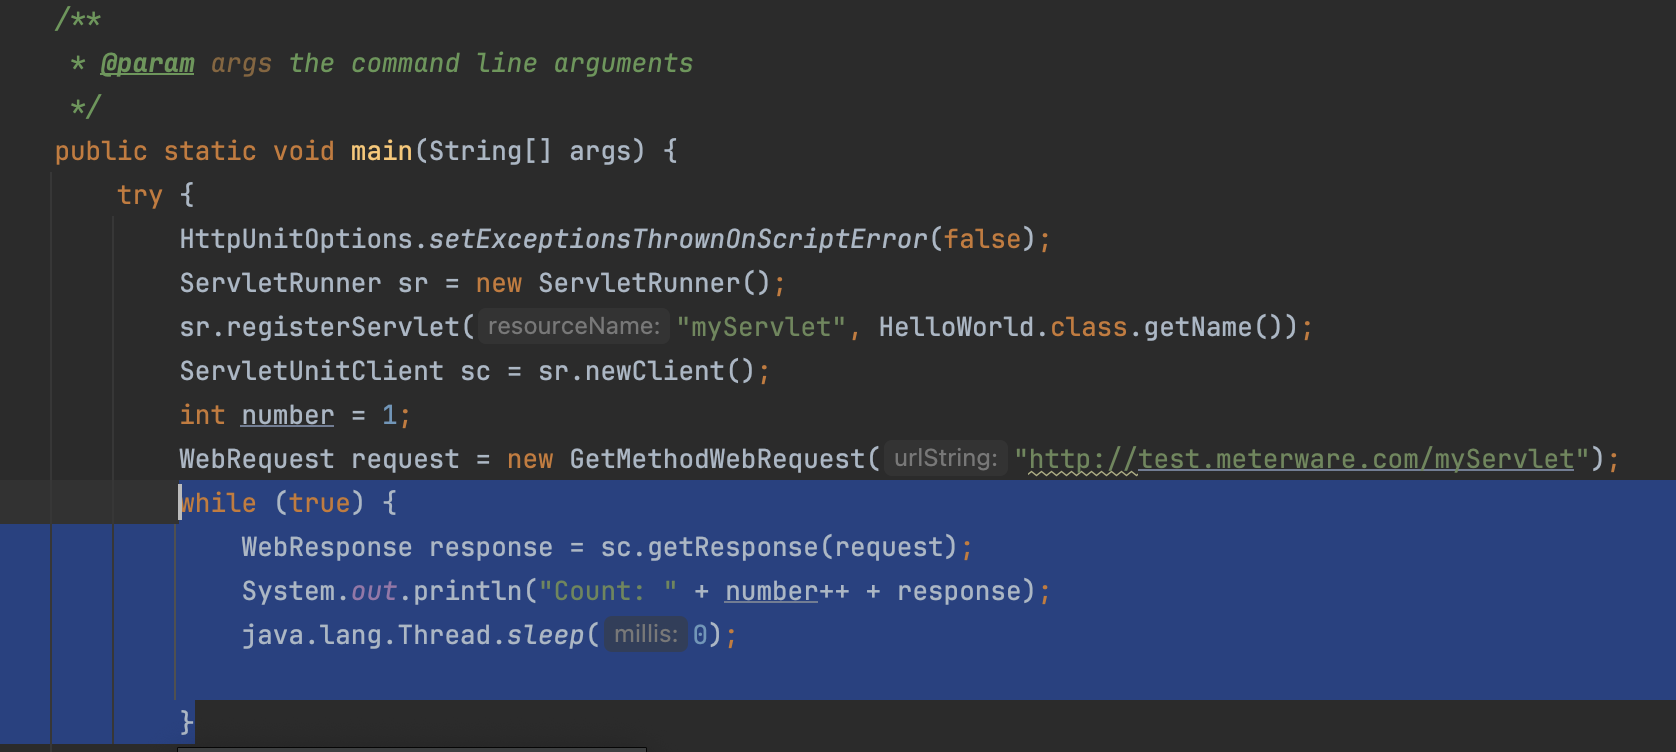
\includegraphics[width=.9\textwidth]{1.png}\\
    \textbf{Скриншот 8. Проблемное место}
\end{center}
Подождал и вылетела ошибка 
\begin{center}
    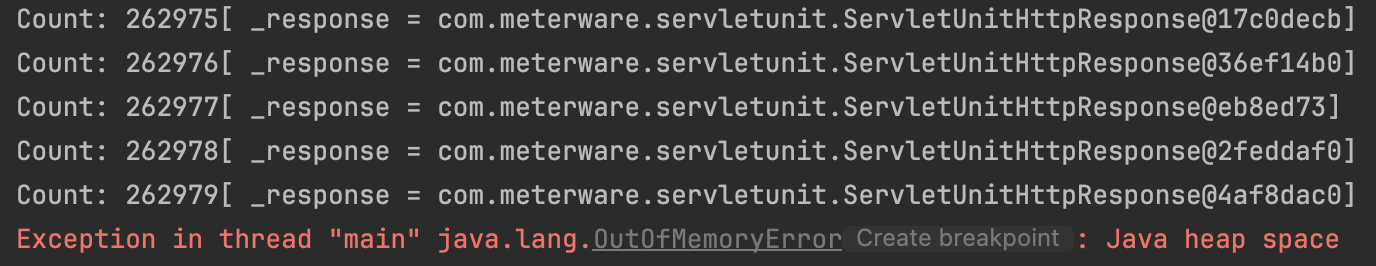
\includegraphics[width=.9\textwidth]{avoska.png}\\
    \textbf{Скриншот 9. Ошибка кучи}
\end{center}
При профилировании уже сразу была видна проблема
\begin{center}
    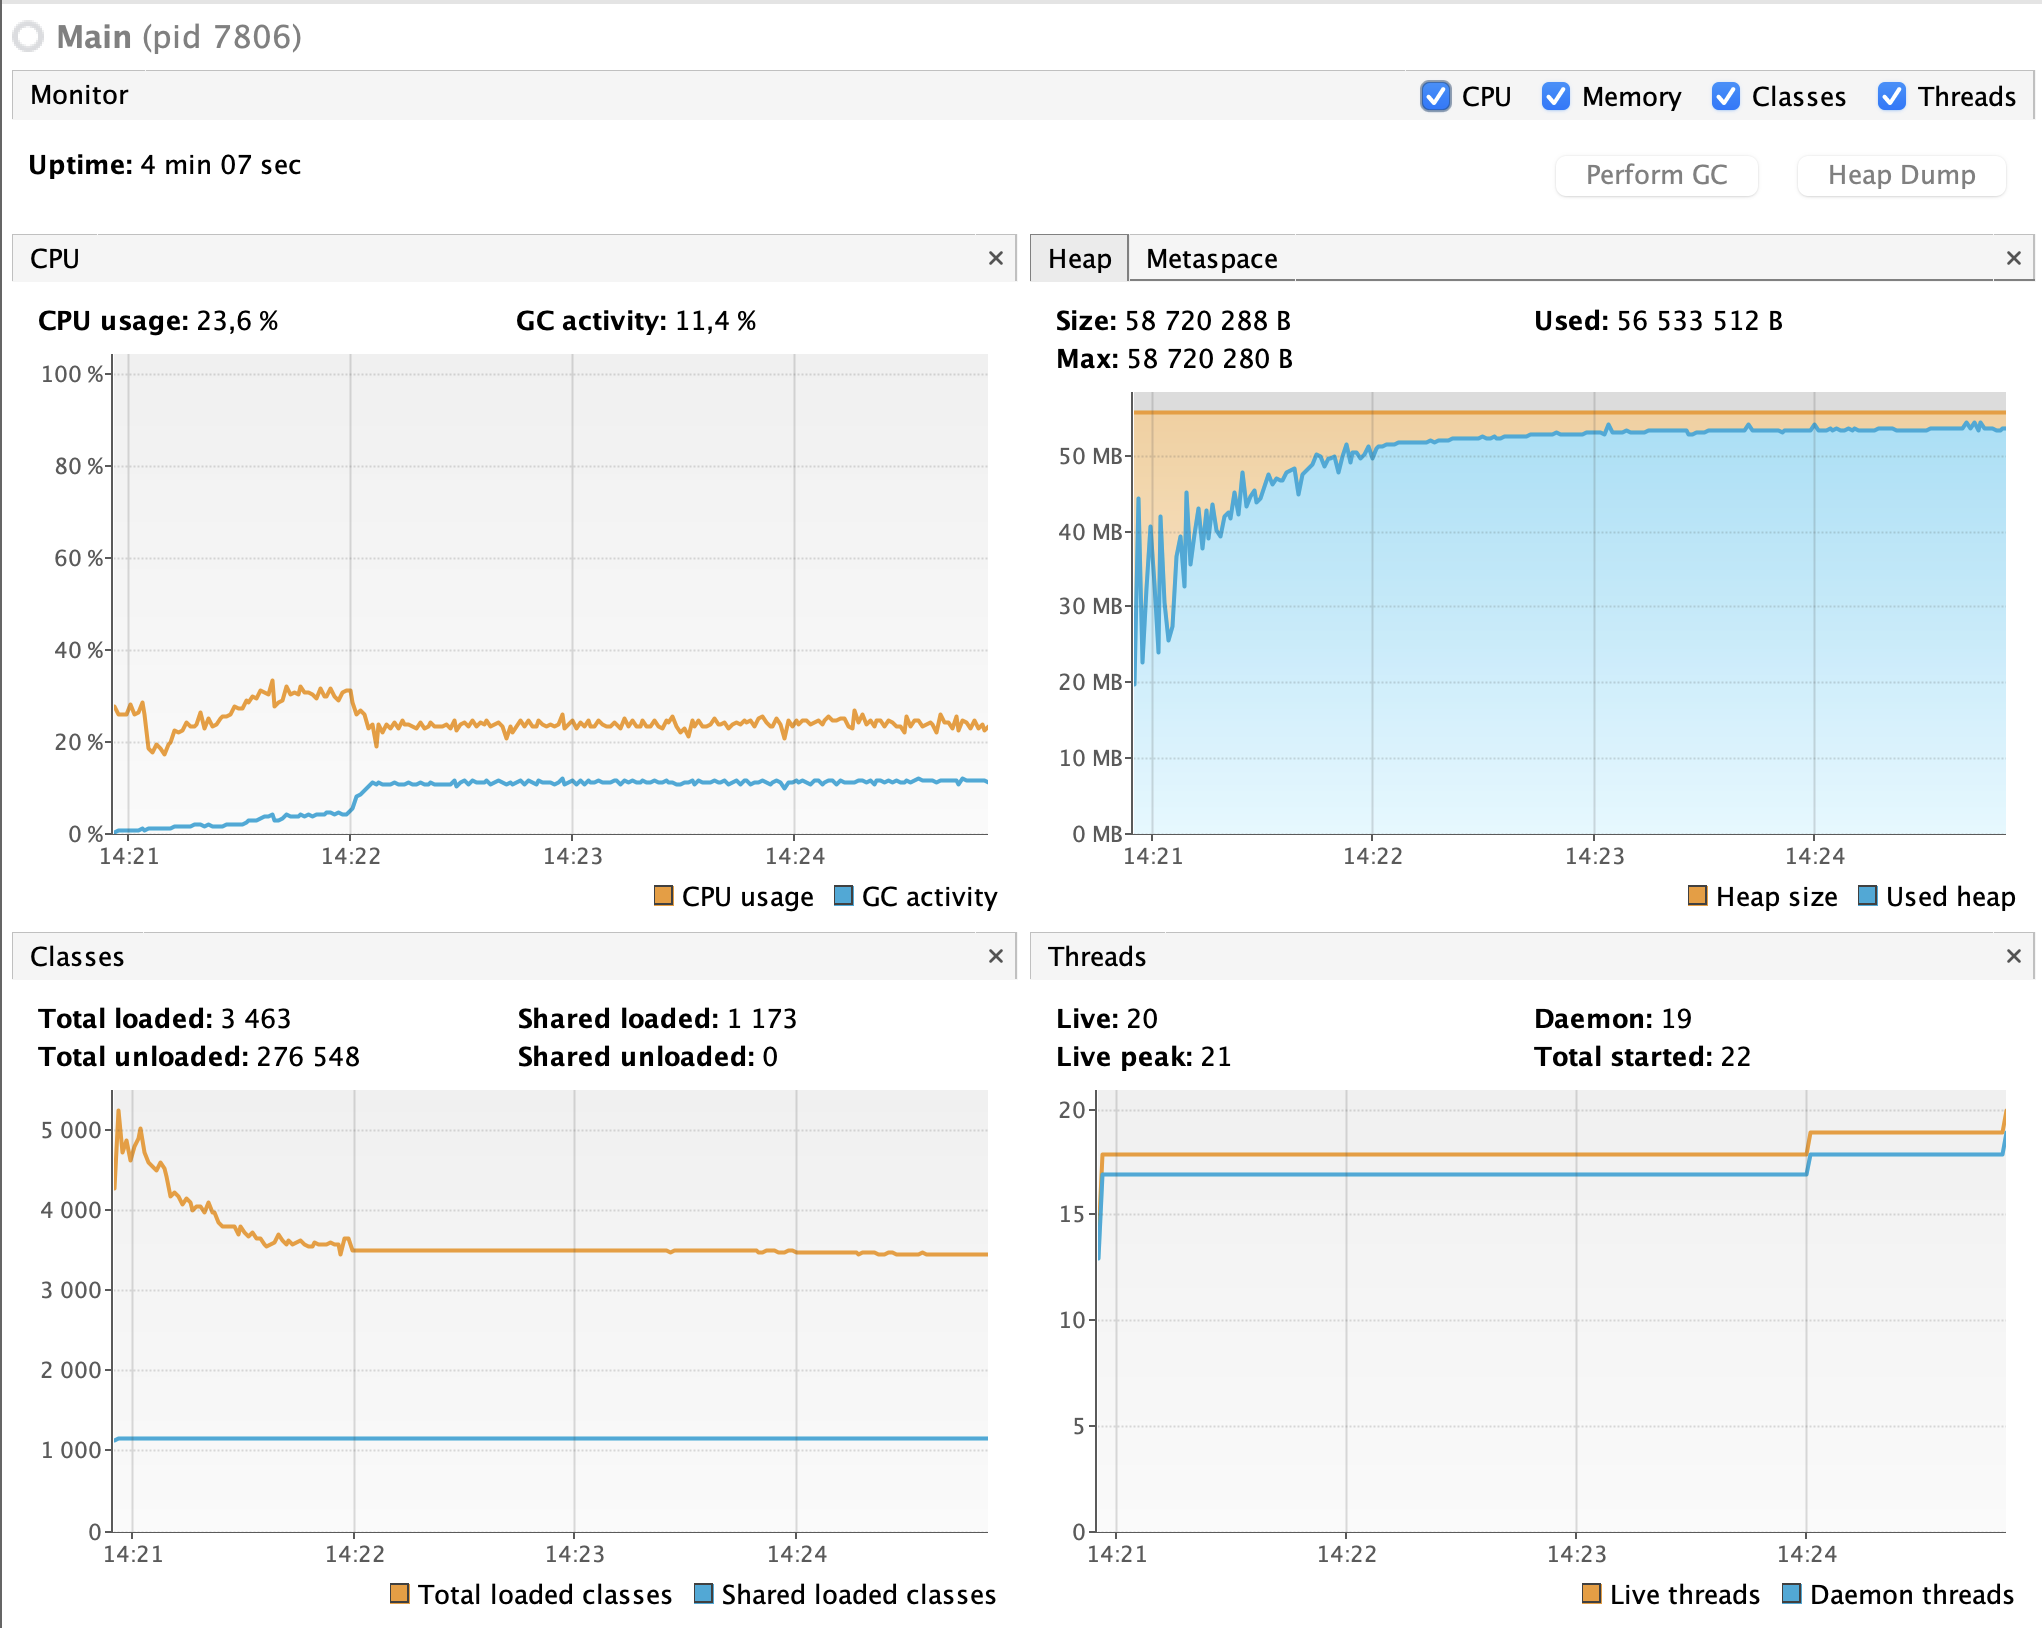
\includegraphics[width=.9\textwidth]{profil.png}\\
    \textbf{Скриншот 10. Ошибка кучи}
\end{center}

Сделал 2 раза HeapDump с небольшим промежутком по времени, чтобы увидеть где подтикает память:
\begin{center}
    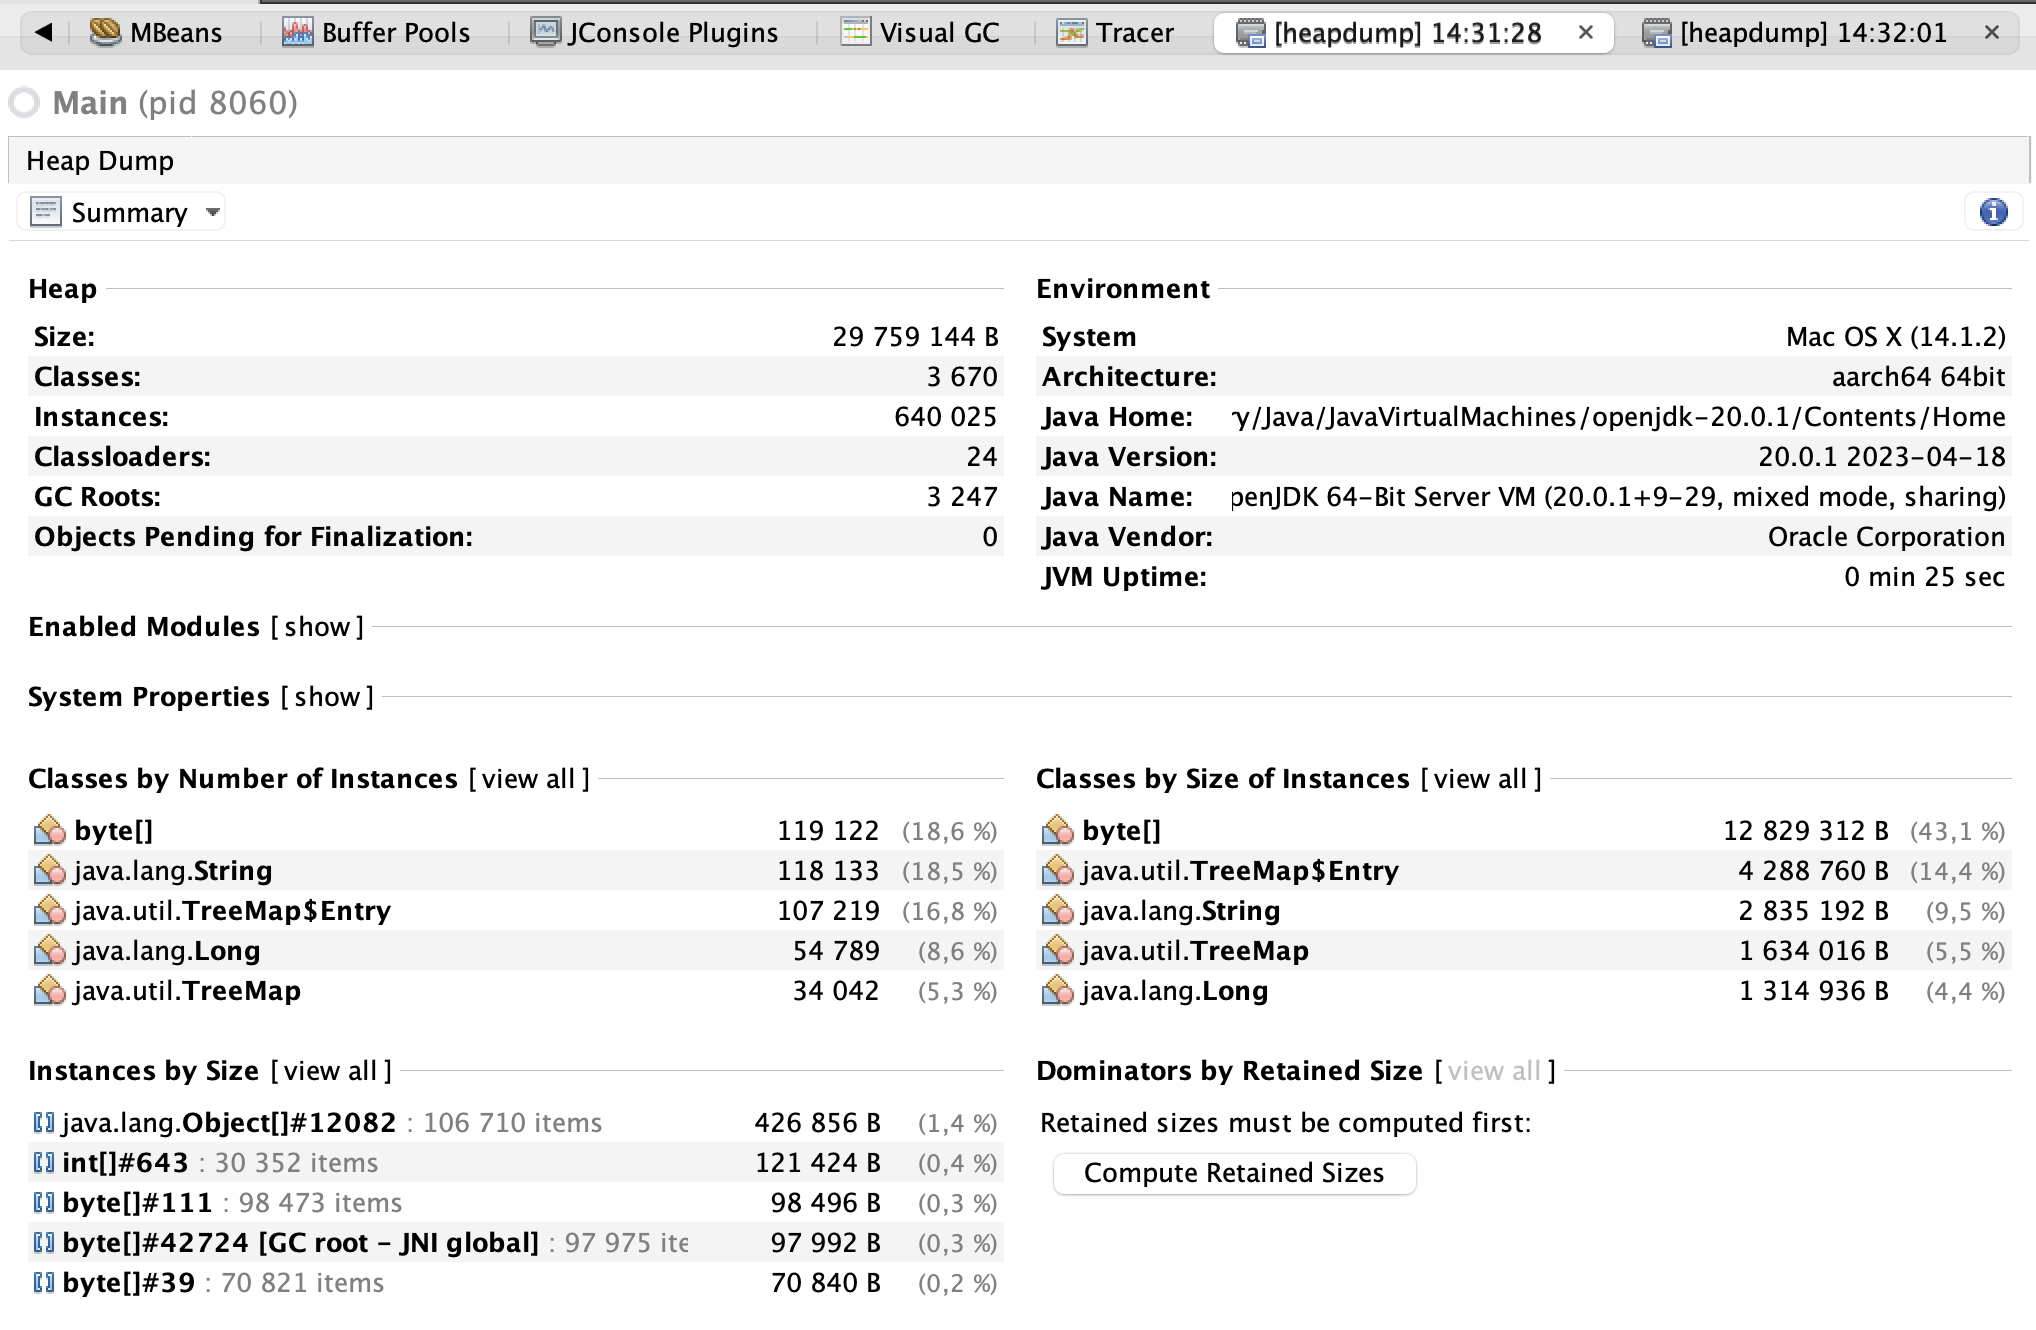
\includegraphics[width=.8\textwidth]{heap1.png}\\
    \textbf{Скриншот 11. Heap Dump}
\end{center}

\begin{center}
    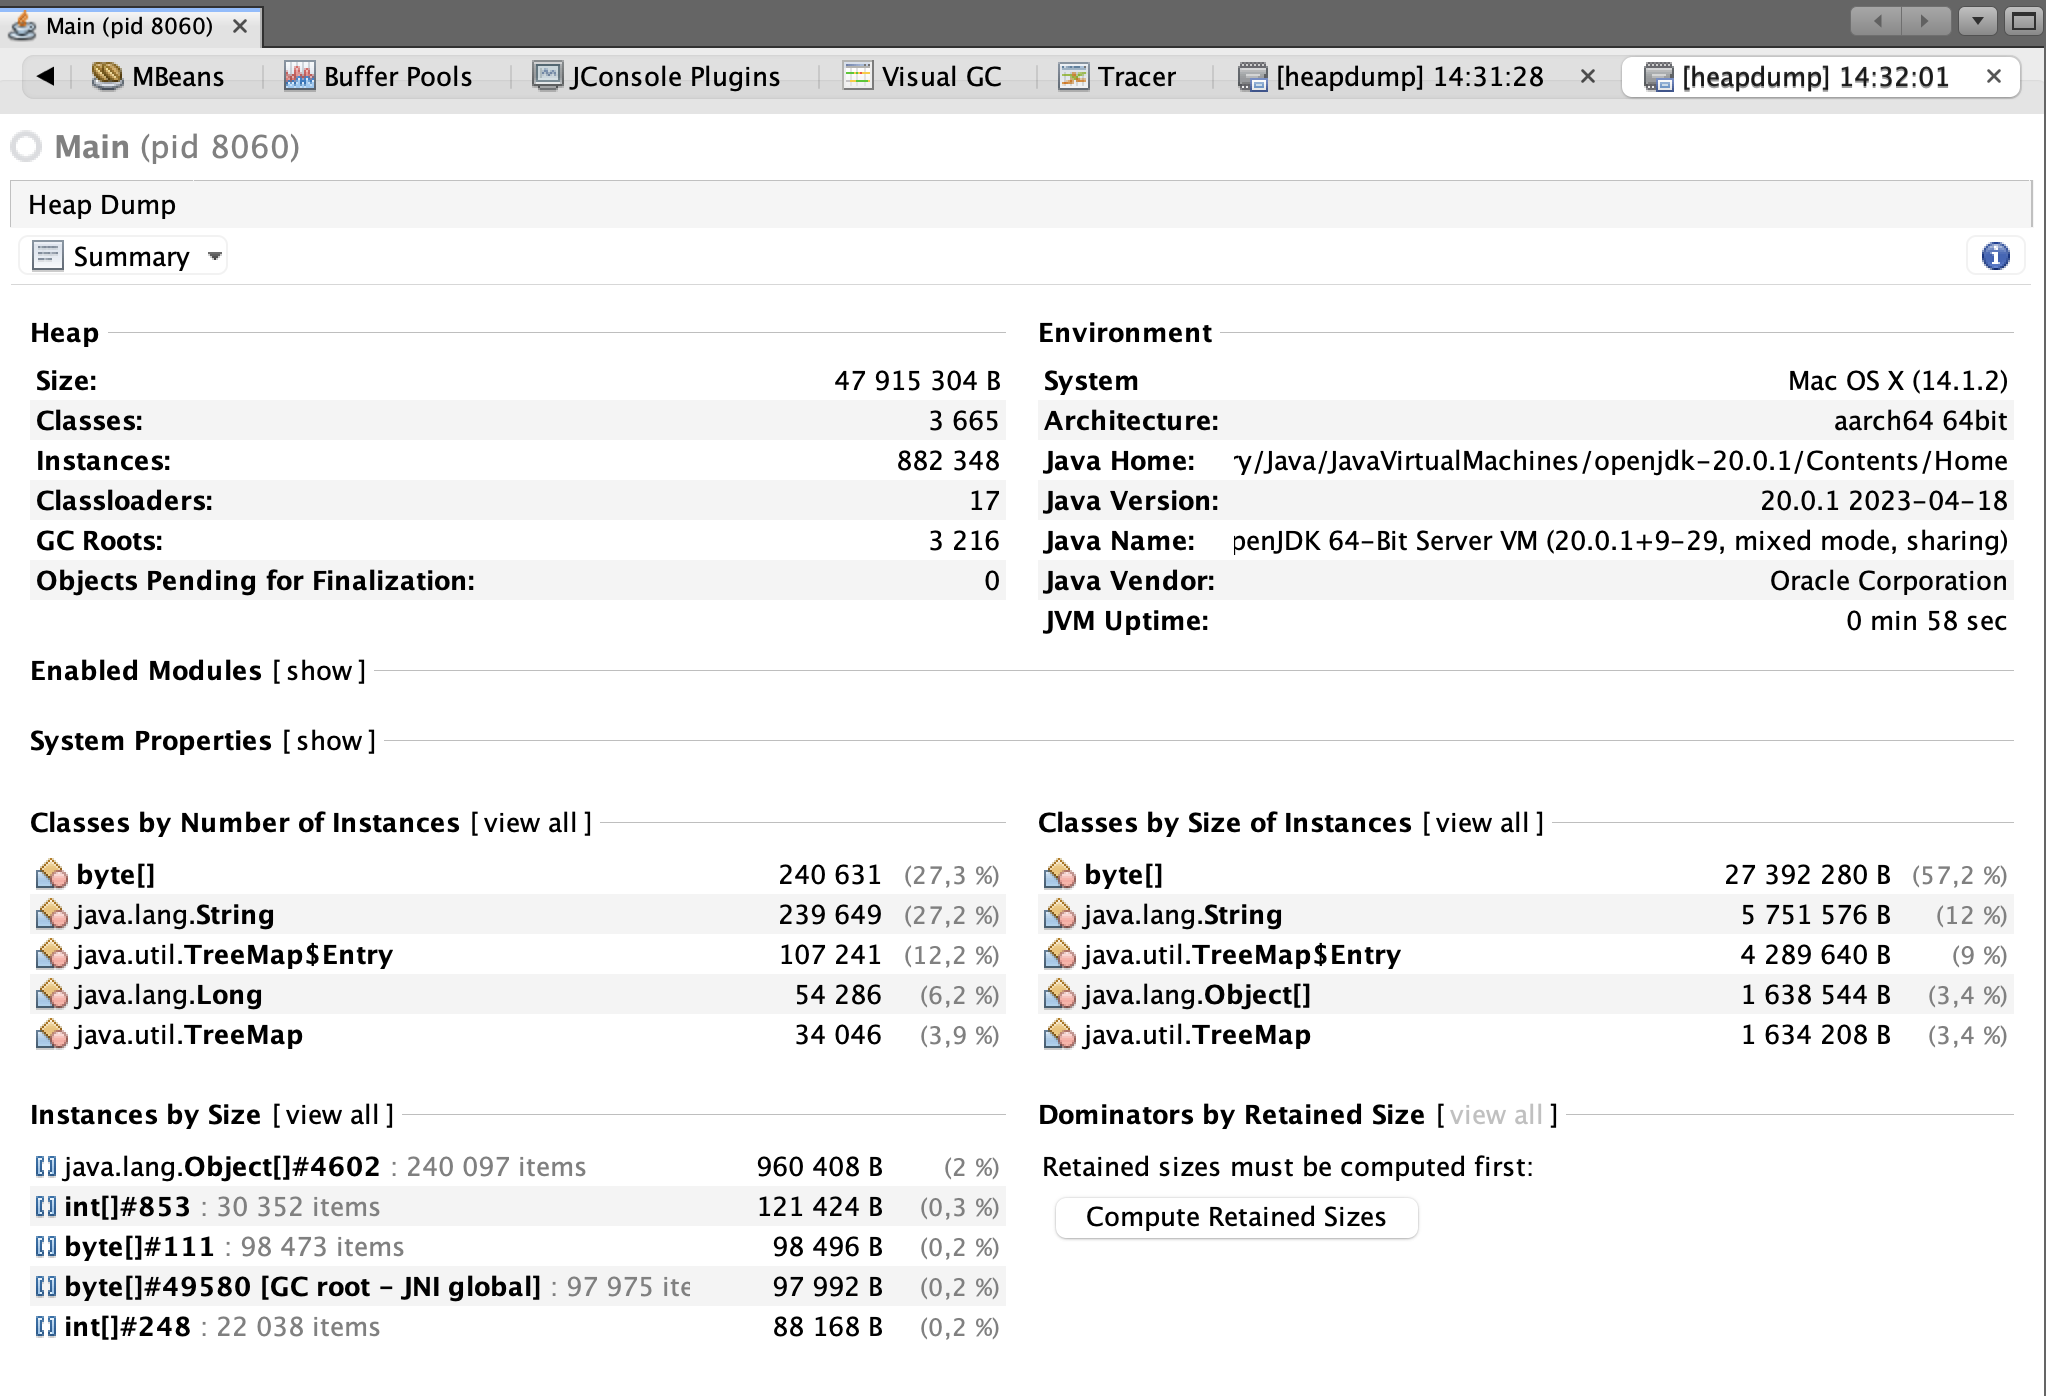
\includegraphics[width=.8\textwidth]{heap2.png}\\
    \textbf{Скриншот 12. Heap Dump}
\end{center}

Нашёл класс из-за которого все проблемы:

\begin{center}
    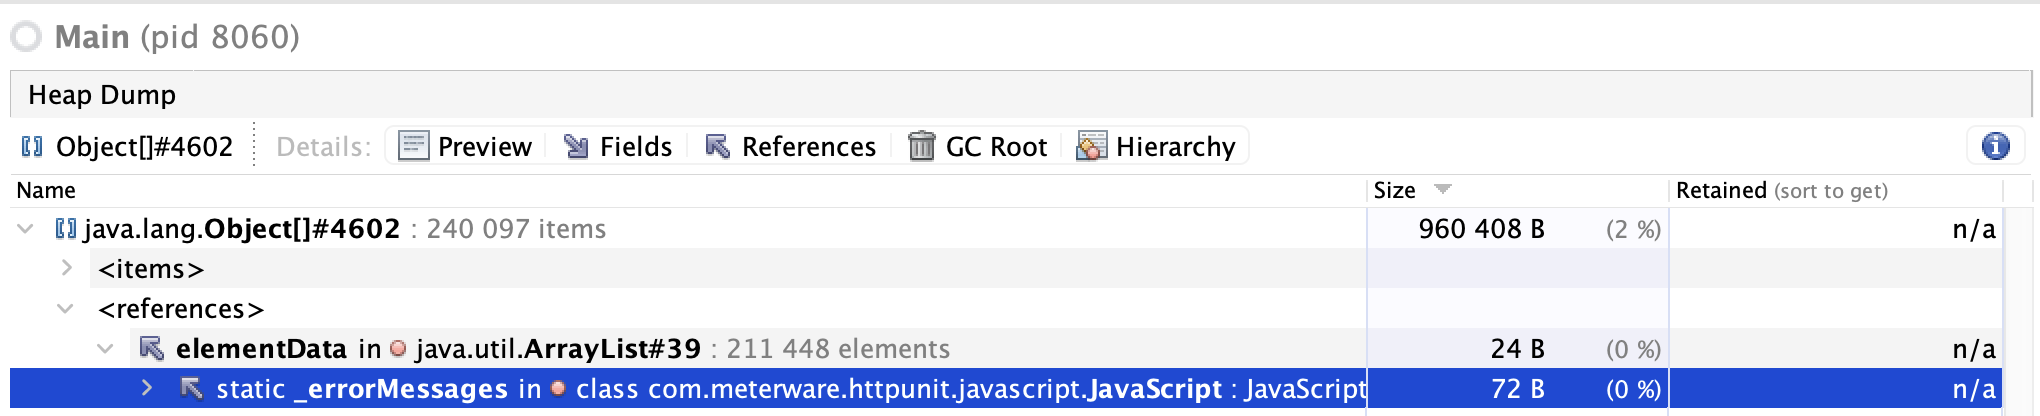
\includegraphics[width=.8\textwidth]{err.png}\\
    \textbf{Скриншот 13. err msg}
\end{center}

В данный список добавление только в одном месте

\begin{center}
    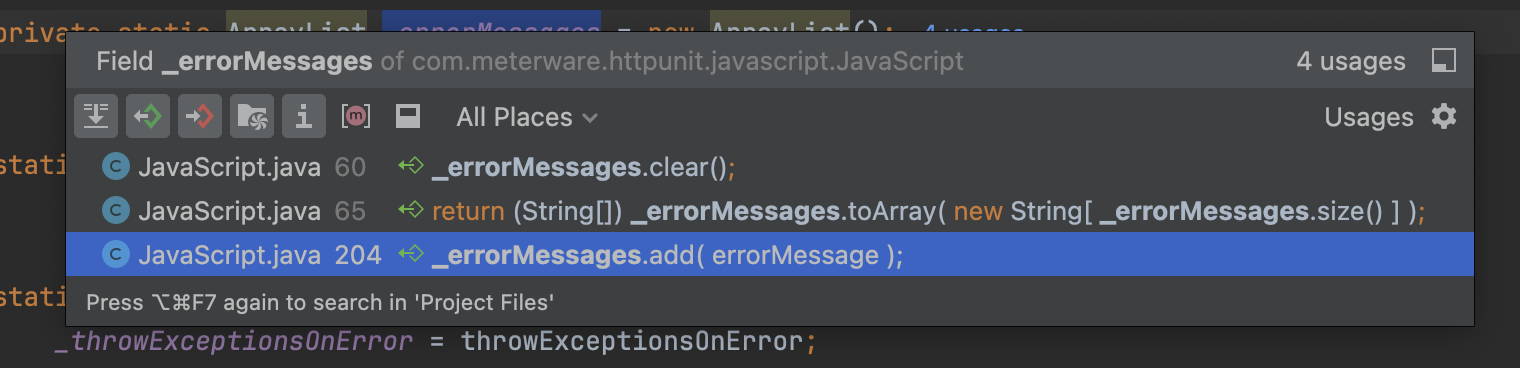
\includegraphics[width=.8\textwidth]{find.png}\\
    \textbf{Скриншот 14. add}
\end{center}

Есть смысл очищать данные при помощи следующего метода:

\begin{center}
    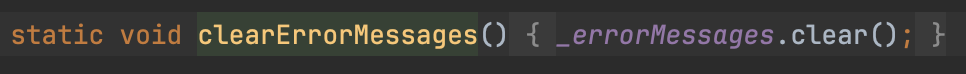
\includegraphics[width=.8\textwidth]{clear.png}\\
    \textbf{Скриншот 15. clear}
\end{center}
\begin{center}
    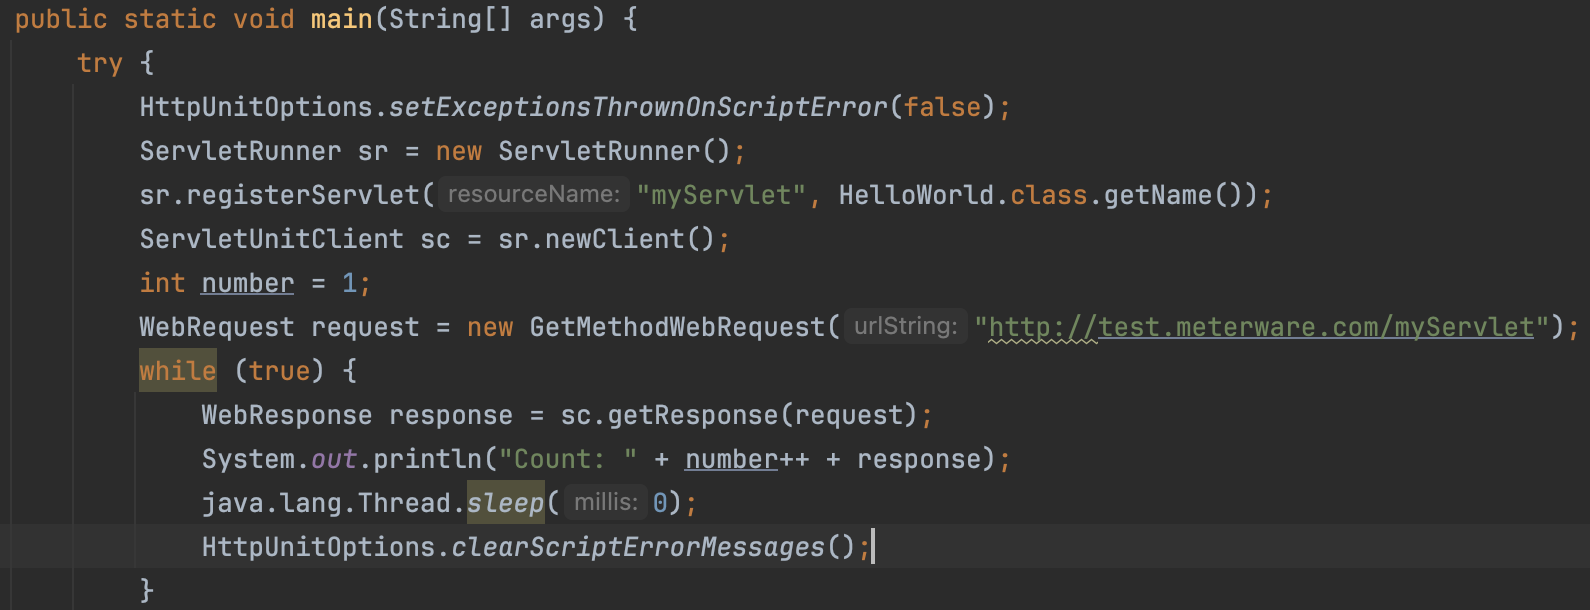
\includegraphics[width=.8\textwidth]{solve.png}\\
    \textbf{Скриншот 16. clear}
\end{center}
После локализации вышел следующий результат
\begin{center}
    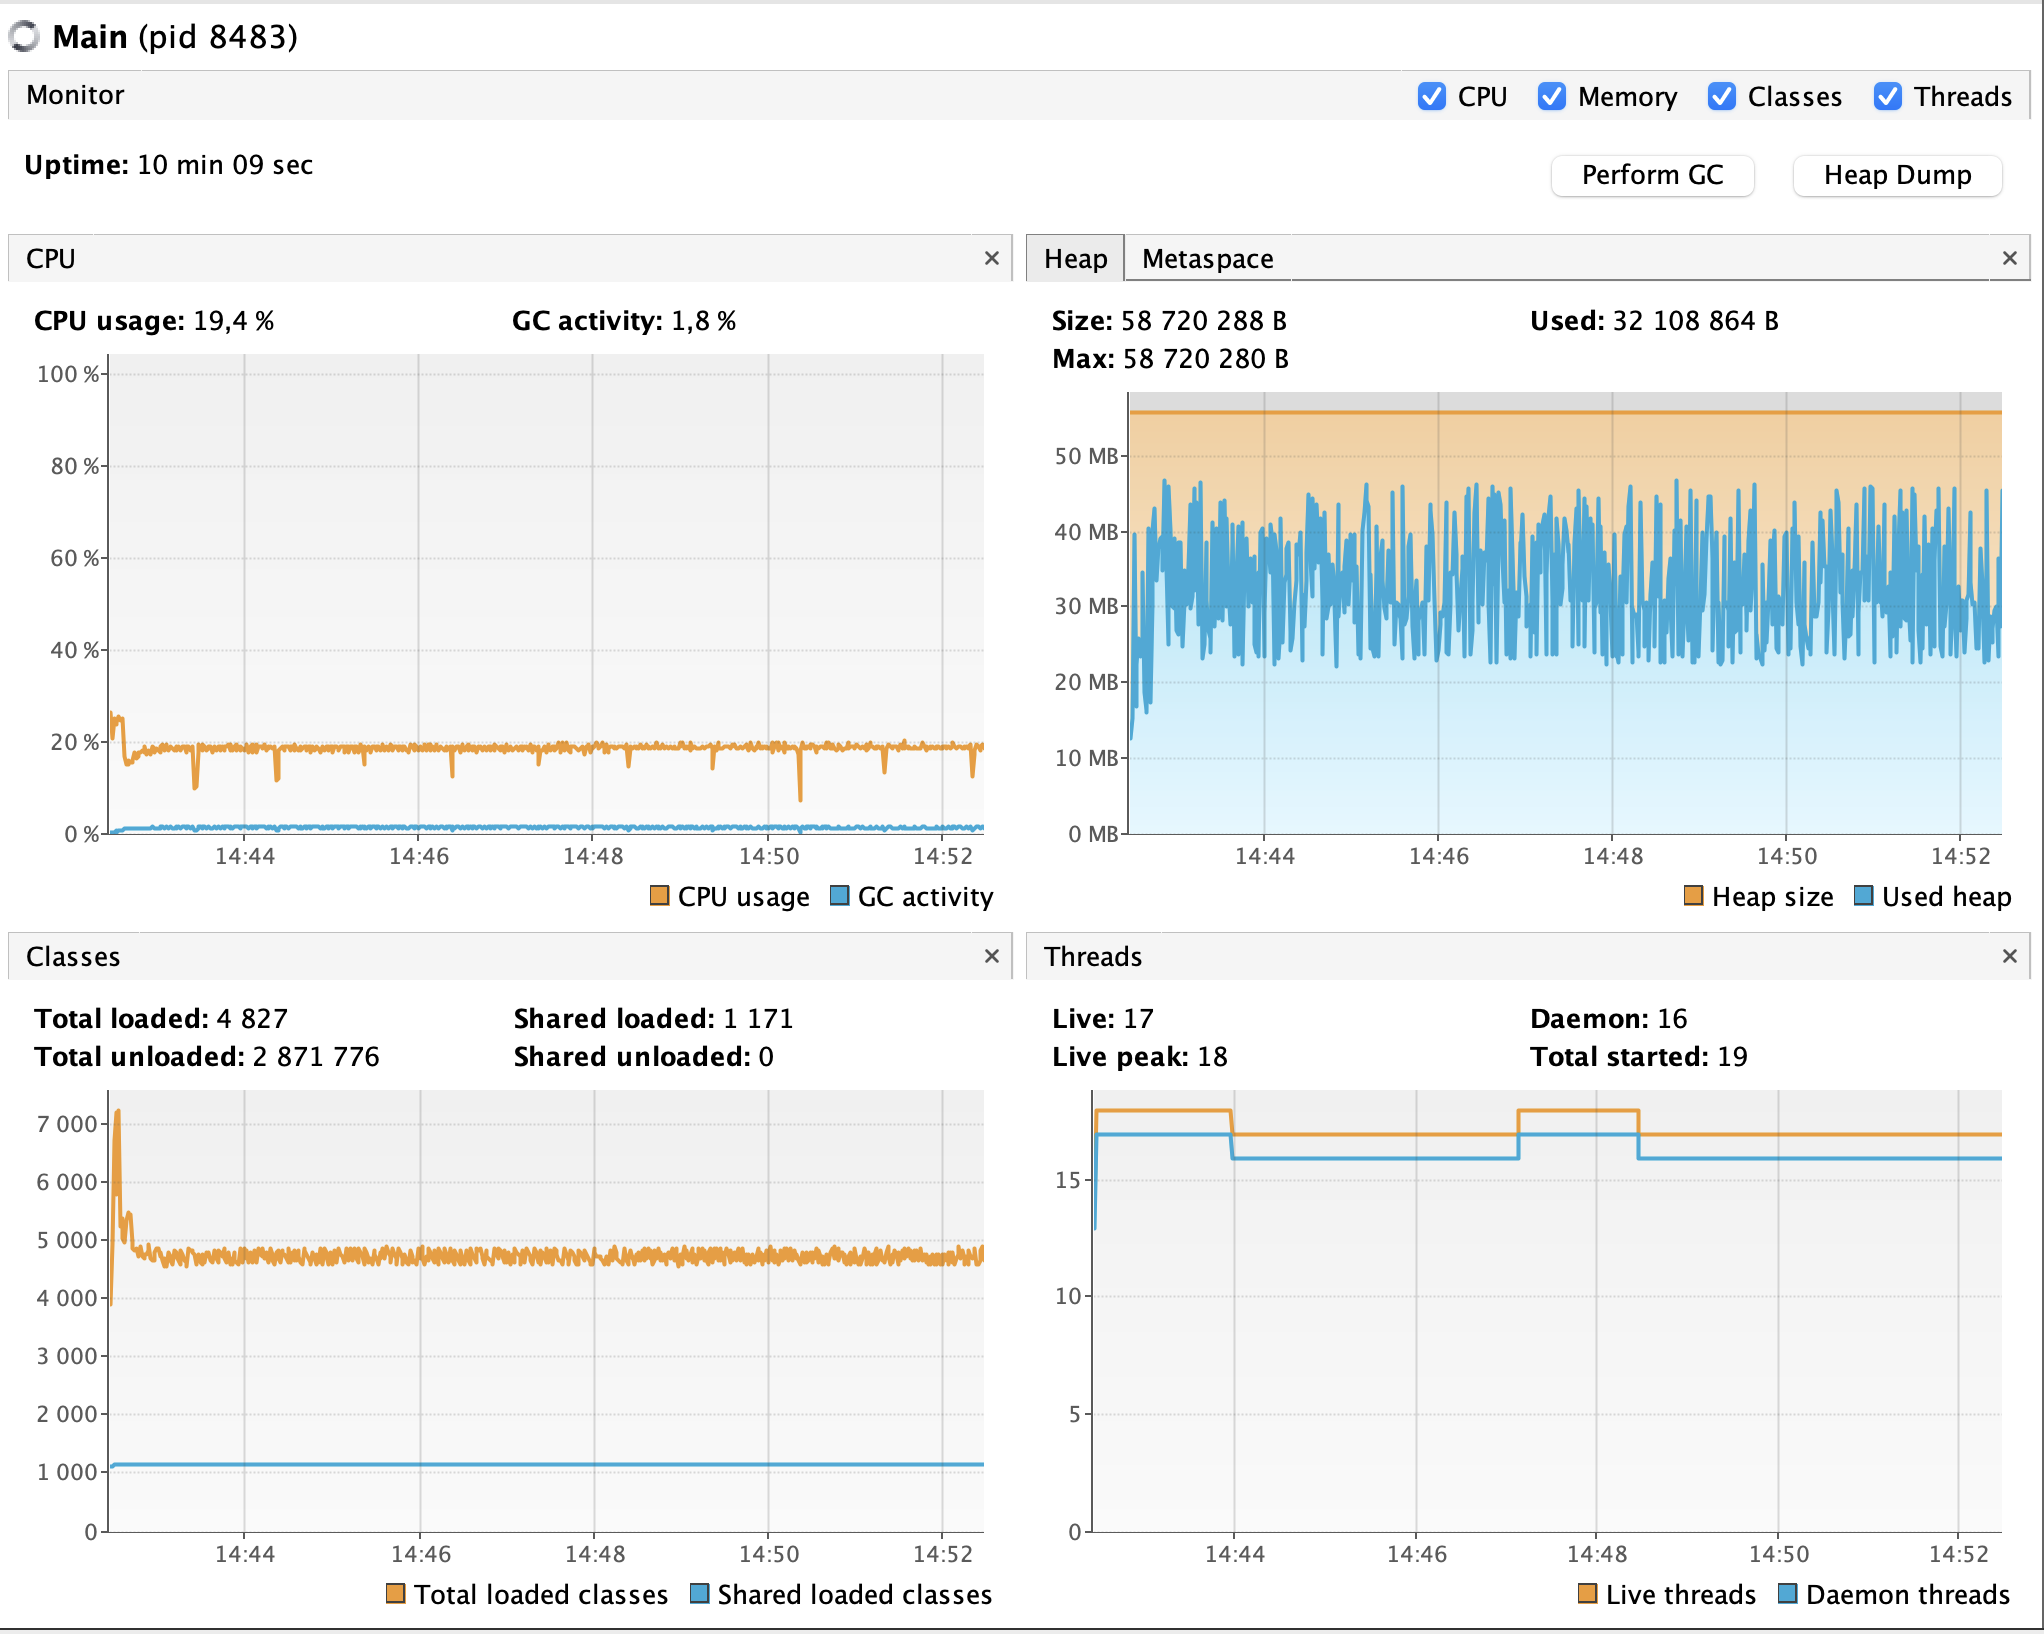
\includegraphics[width=.8\textwidth]{result.png}\\
    \textbf{Скриншот 17. res}
\end{center}
\section{Вывод}
В ходе данной лабораторной работы я ознакомился с утилитами JConsole и VisualVM для мониторинга и профилирования Java приложений. 
Также я научился локализовывать и устранять проблемы, связанные с производительностью приложения.
\end{document}
